\chapter{Design considerations for a heterodyne interferometer}
\label{ch:DesignConsiderations}
While Chapter~\ref{ch:InterferometricMethods} discusses the
\emph{optical} foundations for various interferometric methods,
most real-world optical diagnostics are complex, integrated systems
requiring precise interplay between various components, such as
lasers, optics, detectors, and electronics.
Optimizing the performance of a given diagnostic
requires careful consideration
of each component and its role in the measurement.
Some of these considerations are generic, and
some of them are diagnostic specific.

This chapter examines numerous design considerations
that are relevant to heterodyne interferometry.
The sections are arranged in roughly sequential order,
beginning with the interference signal at the detector and
proceeding through successive downstream components
until reaching the system's digitizer.
In particular, Section~\ref{sec:DesignConsiderations:geometric}
discusses the geometric effects that
affect the magnitude of the heterodyne signal and
set the wavenumber response of the interferometer.
Section~\ref{sec:DesignConsiderations:intensity}
explores heterodyne measurements made
beyond the saturation intensity of a given detector.
Sections~\ref{sec:DesignConsiderations:phase_noise} and
\ref{sec:DesignConsiderations:amplitude_noise}
reveal how phase noise and amplitude noise, respectively,
can creep into the interferometer's measurements.
Section~\ref{sec:DesignConsiderations:demodulation}
describes demodulation of the heterodyne interference signal and
the distortion of the baseband phase signal
that results from demodulator imperfections.
Section~\ref{sec:DesignConsiderations:quantization}
discusses the signal quantization
that necessarily occurs
when generating a digital record.
Finally, for ease of reference,
Section~\ref{sec:DesignConsiderations:summary}
provides a concise summary of the discussed design considerations.
These design considerations will be referenced extensively in
Chapter~\ref{ch:Implementation}, which
describes the addition of a heterodyne interferometer
to the pre-existing phase contrast imaging (PCI) diagnostic
on the \diiid\space tokamak.


\section{Geometric considerations}
\label{sec:DesignConsiderations:geometric}
Several geometric effects substantially influence
the performance of a heterodyne interferometer.
Section~\ref{sec:DesignConsiderations:geometric:aperture_diffraction}
provides a minimum threshold on the radii of components in the optical train,
while Section~\ref{sec:DesignConsiderations:geometric:beam_coalignment}
derives the required degree of coalignment between
the probe beam and the reference beam.
Section~\ref{sec:DesignConsiderations:geometric:beam_mismatch}
discusses the implications of mismatches between
the spatial structures of the probe beam and the reference beam and
develops a criterion for the required level of matching.
Section~\ref{sec:DesignConsiderations:geometric:finite_sampling_volume}
reveals how the imaging system's magnification $M$ and
the detector's size and shape
influence the interferometer's wavenumber response.
Finally, Section~\ref{sec:DesignConsiderations:geometric:depth_of_focus}
examines the depth-of-focus effects that become manifest
when the detector is displaced from the actual image plane.


\subsection{Aperture diffraction}
\label{sec:DesignConsiderations:geometric:aperture_diffraction}
Diffraction from finite-aperture optics was neglected in
Chapter~\ref{ch:InterferometricMethods}'s
transfer-function derivations.
For a propagating Gaussian beam,
this neglect of aperture diffraction is a reasonable approximation if
\begin{equation}
  a_{\text{eff}} \geq \frac{3}{2} w(z),
  \label{eq:DesignConsiderations:aperture_radius_for_minimal_diffraction}
\end{equation}
for each aperture, where
$a_{\text{eff}}$ is the effective aperture radius and
$w(z)$ is the beam's 1/e $E$ radius at the aperture location
\cite{campbell_josa69, rost_diffraction_pc14}.
For a circular aperture of radius $a$,
the effective aperture radius is simply $a_{\text{eff}} = a$
for a beam propagating along the optical axis
(e.g.\ the unscattered beam from
Sec.~\ref{sec:InterferometricMethods:Gaussian_beam_diffraction:from_plasma_density_fluctuations});
however, for a beam located $\rho(z)$ away from the optical axis
(e.g.\ the upscattered or downscattered beam from
Sec.~\ref{sec:InterferometricMethods:Gaussian_beam_diffraction:from_plasma_density_fluctuations}),
the effective aperture radius is $a_{\text{eff}} = a - |\rho(z)|$.


\subsection{Beam coalignment}
\label{sec:DesignConsiderations:geometric:beam_coalignment}
For the moment, assume a plane-wave representation
for both the reference beam and the unscattered probe beam.
Specifically, let the reference beam be given by
\begin{equation}
  \vect{E}_R(\vect{r})
  =
  E_0 \hat{\vect{x}}
  \cdot
  e^{i [k_0 z - (\omega_0 + \Delta \omega_0)t]},
\end{equation}
and let the unscattered probe beam
be misaligned with the reference beam
by angle $\theta \ll 1$ such that,
to lowest order in $\theta$,
the unscattered probe beam is
\begin{equation}
  \vect{E}_P(\vect{r})
  \approx
  E_0 \hat{\vect{x}}
  \cdot
  e^{i [k_0 (z + \theta x) - \omega_0 t]}.
\end{equation}
The total intensity (averaged over an optical cycle) is then
\begin{align}
  I
  =
  \frac{c \varepsilon_0}{2}
  \left|
    \vect{E}_R + \vect{E}_P
  \right|^2
  \approx
  2 I_0 \left[ 1 + \cos(\Delta \omega_0 t + k_0 \theta x) \right],
\end{align}
where $I_0 = c \varepsilon_0 E_0^2 / 2$
is the corresponding intensity of a single beam.
Here, the cosine term
corresponds to the interference between the two beams, and
the unity term corresponds to the intensity of each individual beam.
Optimizing the interference signal requires
alignment of the beam polarizations and
minimization of the misalignment angle $\theta$.
If the interference is measured by a detector
with an extent $s_x$ in the $x$-direction,
the misalignment-induced phase $k_0 \theta x$
should change by much less than $2 \pi$ across the detector face;
i.e.\ $|k_0 \theta s_x| \ll 2 \pi$ or
\begin{equation}
  |\theta|
  \ll
  \frac{\lambda_0}{s_x}
  \approx
  0.6^{\circ},
  \label{eq:DesignConsiderations:coalignment_constraint}
\end{equation}
where $\lambda_0 = 2 \pi / k_0$ is the beam wavelength, and
$\lambda_0 = \SI{10.6}{\micro\meter}$ and
$s_x = \SI{1}{\milli\meter}$
have been used for the evaluation.
While coalignment constraint
(\ref{eq:DesignConsiderations:coalignment_constraint})
is relatively easy to satisfy during a system alignment,
it does have design implications for CO$_2$ interferometers
that are built for magnetic fusion experiments, which
are often characterized by large, pulsed electromagnets
whose operation may contort the machine and produce vibrations,
potentially destroying the beam coalignment.


\subsection{Mismatch between beam spatial structures}
\label{sec:DesignConsiderations:geometric:beam_mismatch}
The external reference-beam interferometry derivations
in Section~\ref{sec:InterferometricMethods:interferometry}
assumed that the reference beam was exactly matched
in both amplitude and spatial structure
to the unscattered probe beam.
This is obviously an idealization
that, at best, can only be approximately met in experiment.
This section discusses the geometric effects
of such imperfections in beam matching.

The derivation of the heterodyne intensity
(\ref{eq:InterferometricMethods:heterodyne_intensity})
can be easily generalized to account for
the geometric effects of unmatched reference and probe beams.
Namely, let the image-plane probe radiation be given by
(\ref{eq:InterferometricMethods:imaged_total_field_interferometer}) as
\begin{equation}
  E_P(\vect{r}_{\image}, t)
  \approx
  E_{G,P}(\vect{r}_{\image}, t)
  e^{i \bar{\phi}}
  \left[%
    1
    +
    i \tilde{\phi}(x_{\image}, t)
  \right],
\end{equation}
and let the corresponding reference beam be given by
\begin{equation}
  E_R(\vect{r}_{R}, t)
  =
  E_{G,R}(\vect{r}_{R}, t) e^{-i \Delta\omega_0 t},
\end{equation}
where $\vect{r}_{\image} = (x_{\image}, y_{\image}, z_{\image})$,
\begin{equation}
  \vect{r}_{R}
  =
  \vect{r}_{\image}
  +
  (0, 0, z_{R} - z_{\image}),
\end{equation}
and $E_{G,j}$ is a Gaussian beam
with angular frequency $\omega_0$,
waist amplitude $E_{0,j}$, and
waist 1/e $E$ radius $w_{0,j}$.
If $z_R \neq z_{\image}$,
the reference beam's waist sits at a different location
than that of the unscattered probe beam.
Under these circumstances and to first order in $\tilde{\phi}$,
the heterodyne intensity (averaged over an optical cycle) becomes
\begin{equation}
  \begin{aligned}
    I_{\text{het}}(\vect{r}_{\image}, z_R, t)
    &=
    I_{\text{DC}}
    +
    I_{\text{AC}}
    \cos(\Delta \omega_0 t + \bar{\phi}_{\text{eff}})
    \\
    &\quad-
    I_{\text{AC}}
    \tilde{\phi}(x_{\image}, t)
    \sin(\Delta \omega_0 t + \bar{\phi}_{\text{eff}}),
  \end{aligned}
  \label{eq:DesignConsiderations:heterodyne_intensity}
\end{equation}
where
\begin{align}
  I_{\text{DC}}
  &=
  I_{G,P}(\vect{r}_{\image}) + I_{G,R}(\vect{r}_R),
  \label{eq:DesignConsiderations:I_DC}
  \\
  I_{\text{AC}}
  &=
  2 \sqrt{I_{G,P}(\vect{r}_{\image}) \cdot I_{G,R}(\vect{r}_R)}
  \label{eq:DesignConsiderations:I_AC}
\end{align}
are the DC and AC components of the heterodyne intensity, respectively,
\begin{equation}
  I_{G,j}(\vect{r})
  =
  \frac{c \varepsilon_0 |E_{G,j}(\vect{r})|^2}{2}
\end{equation}
is the intensity profile (averaged over an optical cycle)
of Gaussian beam $j \in \{P, R\}$,
\begin{equation}
  \bar{\phi}_{\text{eff}}
  =
  \bar{\phi}
  +
  \bigl[ \phi_{G,P}(\vect{r}_{\image}) - \phi_{G,R}(\vect{r}_R) \bigr]
\end{equation}
is the effective bulk phase, and
\begin{equation}
  \phi_{G,j}(\vect{r})
  =
  k_0 z + \frac{k_0 \rho^2}{2 R_j(z)} - \psi_j(z)
\end{equation}
is the phase of Gaussian beam $j \in \{P, R\}$
(i.e.\ $E_{G,j}(\vect{r}) = |E_{G,j}(\vect{r})| e^{i \phi_{G,j}(\vect{r})}$).
Note that (\ref{eq:DesignConsiderations:heterodyne_intensity})
readily reduces to (\ref{eq:InterferometricMethods:heterodyne_intensity})
if $E_{G,R}(\vect{r}_R) = E_{G,P}(\vect{r}_{\image})$.

It is worth discussing the implications of heterodyne intensity
(\ref{eq:DesignConsiderations:heterodyne_intensity}).
First, repeating the derivation between
(\ref{eq:InterferometricMethods:heterodyne_interferometer_I_and_Q_intensity})
and
(\ref{eq:InterferometricMethods:heterodyne_interferometer_wavenumber_transfer_function})
with this modified heterodyne intensity,
one readily finds that
the heterodyne interferometer's wavenumber transfer function
(\ref{eq:InterferometricMethods:heterodyne_interferometer_wavenumber_transfer_function})
should be multiplied by the factor
$2 I_{\text{AC}} / (I_{\text{DC}} + I_{\text{AC}})$.
It is then easy to show that
the transfer function is \emph{maximized} when
$I_{\text{DC}} = I_{\text{AC}}$,
i.e.\ when the probe beam and reference beam
have identical spatial structures and powers.
Second, note that the effective bulk phase $\bar{\phi}_{\text{eff}}$
is dependent on the geometry of the reference beam and
the unscattered probe beam.
Specifically, in the context of measuring
the plasma-induced bulk phase $\bar{\phi}$,
note that
\begin{equation}
  \bar{\phi}_{\text{eff}}(\rho_{\image}=0)
  =
  \bar{\phi}
  +
  k_0 (z_{\image} - z_R)
  -
  \left[ \psi_P(z_{\image}) - \psi_R(z_R) \right].
\end{equation}
If $z_{\image}$ and $z_R$ are fixed,
then the beam-geometry contributions to
$\bar{\phi}_{\text{eff}}(\rho_{\image} = 0)$
constitute an unimportant DC offset that can be removed
via baseline subtraction;
however, experiments are typically plagued by vibrations, and
even small changes to $z_{\image}$ and $z_R$
can make significant time-dependent contributions to
$\bar{\phi}_{\text{eff}}(\rho_{\image} = 0)$ at CO$_2$ probe wavelengths.
As such, deconvolving the plasma-induced and vibration-induced contributions
to $\bar{\phi}_{\text{eff}}(\rho_{\image} = 0)$
requires interferometric measurements
at two distinct wavelengths (i.e.\ two-color interferometry)
\cite{carlstrom_rsi88}.
However, such vibrations occur on slow time-scales
(e.g.\ $f_{\text{vib}} \lesssim \SI{5}{\kilo \hertz}$),
and phase measurements at a \emph{single} wavelength are sufficient
to quantify plasma-induced phase fluctuations
at frequencies above $f_{\text{vib}}$
\cite{vanzeeland_ppcf05}.
Finally, note that the beam geometry also imparts
a spatially dependent, curvature-induced phase shift
\begin{align}
  \delta\phi_{\kappa}(\rho_{\image})
  &=
  \bar{\phi}_{\text{eff}}(\rho_{\image})
  -
  \bar{\phi}_{\text{eff}}(\rho_{\image} = 0)
  \notag \\
  &=
  \frac{k_0 \rho_{\image}^2}{2}
  \left[\frac{1}{R_P(z_{\image})} - \frac{1}{R_R(z_R)} \right],
\end{align}
which can result in signal loss and distortion of the measured wavenumber.
To see this, assume that the radiation is interfered on a detector array,
as shown in Figure~\ref{fig:DesignConsiderations:detector_array}.
As a detector element produces a signal
proportional to the average intensity across its face,
there will be substantial signal loss
if there are large curvature-induced phase shifts
across the element's face
(i.e.\ $\delta\phi_{\kappa}(s_x / 2) \gtrsim \pi$ or
$\delta\phi_{\kappa}(s_y / 2) \gtrsim \pi$).
Further, if there are large curvature-induced phase shifts
across the length of the detector array,
the spatial structure of the intensity
will \emph{not} correspond to the spatial structure
of the plasma fluctuation.
The latter is the more conservative constraint
on the curvature-induced phase shift.
Assuming that the detector array shown in
Figure~\ref{fig:DesignConsiderations:detector_array}
consists of $N_{\text{el}}$ detector elements and
that the inter-element spacing is negligible ($\delta_x \ll s_x$),
the criterion for negligible curvature-induced phase shifts
$\text{max}(\delta\phi_{\kappa})
=
\delta\phi_{\kappa}(\rho_{\image, \text{max}})
\ll
\pi$
becomes
\begin{equation}
  \text{max}(\delta\phi_{\kappa})
  =
  \frac{k_0}{8}
  \left[ (N_{\text{el}} s_x)^2 + s_y^2 \right]
  \left| \frac{1}{R_P(z_{\image})} - \frac{1}{R_R(z_R)}\right|
  \ll
  \pi.
\end{equation}

\begin{figure}
  \centering
  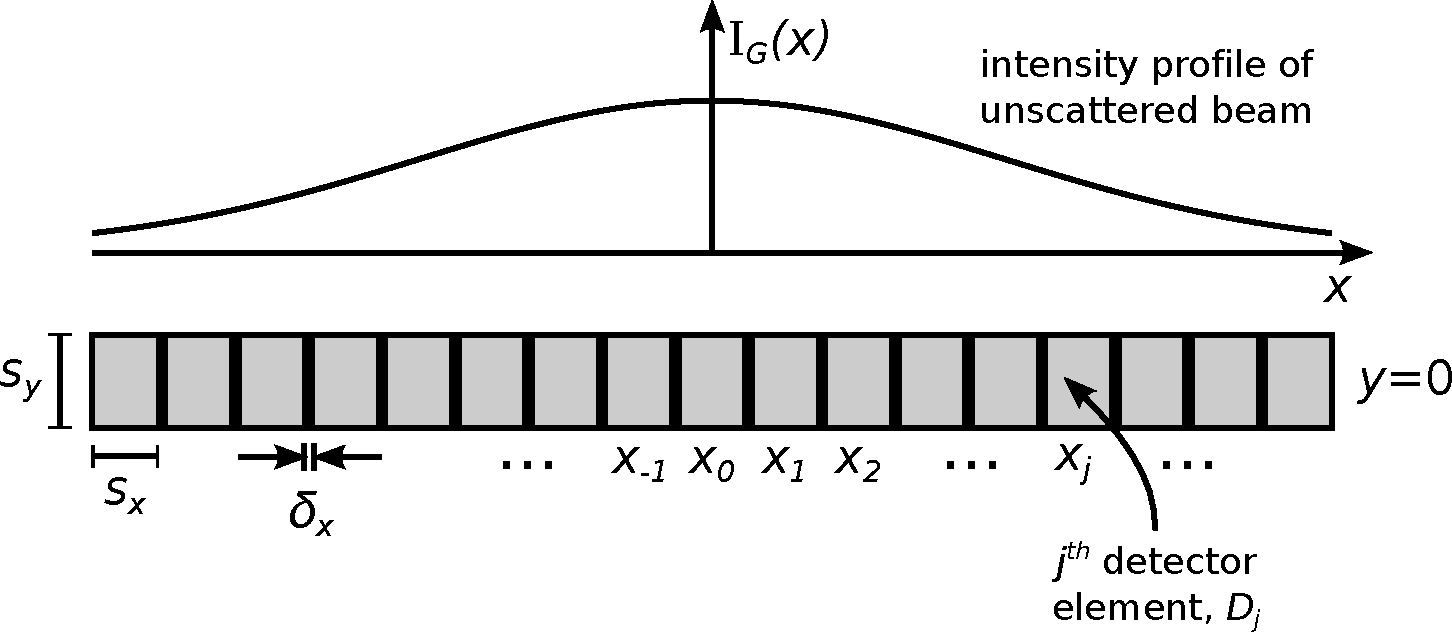
\includegraphics[width = \textwidth]{%
    Chapters/DesignConsiderations/figs/detector_array.pdf}
  \caption[Finite sampling volumes in a detector array]{%
    The probe radiation and the reference beam
    are interfered on a detector array.
    The array consists of numerous detector elements,
    each of size $s_x \times s_y$ and with interelement spacing $\delta_x$.
    The unscattered beam is centered on $x = x_0$ and $y = 0$, and
    its intensity profile varies only weakly over any given element.
    The finite size of each detector element tends to attenuate
    short wavelength components of the incident optical signal.
  }
\label{fig:DesignConsiderations:detector_array}
\end{figure}


\subsection{Finite sampling-volume effects}
\label{sec:DesignConsiderations:geometric:finite_sampling_volume}
Practically speaking, detection is always effected
via detector elements of \emph{finite} size,
with the output of each detector element
corresponding to the incident intensity
\emph{averaged} over the element's active area.
This averaging acts as a low-pass filter in the spatial domain and
is referred to as the finite sampling-volume effect~\cite{bravenec_rsi95}.

Finite sampling-volume effects dictate
a heterodyne interferometer's wavenumber response~\cite{davis_rsi16}.
To see this, assume that measurements
are made with the array of rectangular detector elements shown in
Figure~\ref{fig:DesignConsiderations:detector_array}
(for circular elements, see Coda's discussion~\cite[Sec.~3.7]{coda_phd}).
Let the $j$\ts{th} detector element $D_j$ be centered on $x_{\image,j}$
and $y_{\image} = 0$.
Integrating the optical intensity $\tilde{I}_{IQ}(\vect{r}_{\image}, t)$
corresponding to fluctuations in the baseband signal from
(\ref{eq:InterferometricMethods:heterodyne_total_fluctuating_intensity})
over the face of detector element $D_j$ yields
the corresponding optical power
\begin{align}
  \tilde{P}_{IQ,j}(t)
  &=
  \int_{D_j} \tilde{I}_{IQ}(\vect{r}_{\image}, t) dA
  \notag \\
  &\approx
  \frac{2 \sqrt{2}}{\pi}
  I_G(\vect{r}_{\image,j}) s_y
  \int_{x_{\image,j} - s_x / 2}^{x_{\image,j} + s_x / 2}
  \tilde{\phi}(x_{\image}, t)
  dx_{\image};
  \label{eq:DesignConsiderations:fluctuating_baseband_equivalent_optical_power_per_element_v1}
\end{align}
here, the intensity profile $I_G(\vect{r}_{\image})$
has been assumed to be approximately constant
over the face of the detector element.
Because (\ref{eq:DesignConsiderations:fluctuating_baseband_equivalent_optical_power_per_element_v1})
is linear in $\tilde{\phi}$,
it is suitable to consider a single Fourier mode
\begin{equation}
  \tilde{\phi}(x_{\image}, t)
  =
  \tilde{\phi}_0 \cos(k_{\image} x_{\image} - \omega t)
\end{equation}
for which (\ref{eq:DesignConsiderations:fluctuating_baseband_equivalent_optical_power_per_element_v1})
reduces to
\begin{equation}
  \tilde{P}_{IQ,j}(t)
  =
  \frac{2 \sqrt{2}}{\pi}
  I_G(\vect{r}_{\image,j}) A
  \cdot
  T_{\text{fsv}}(k_{\image})
  \cdot
  \tilde{\phi}_0 \cos(k_{\image} x_{\image} - \omega t),
  \label{eq:DesignConsiderations:fluctuating_baseband_equivalent_optical_power_per_element_v2}
\end{equation}
where $A = s_x s_y$ is the area of the detector element,
\begin{equation}
  T_{\text{fsv}}(k_{\image})
  \equiv
  \sinc\left( \frac{k_{\image}}{k_{\text{fsv},\image}} \right)
  \label{eq:DesignConsiderations:finite_sampling_volume_transfer_function}
\end{equation}
is the finite sampling-volume transfer function,
\begin{equation}
  \sinc(x) = \frac{\sin(\pi x)}{\pi x}
  \label{eq:DesignConsiderations:normalized_sinc}
\end{equation}
is the normalized sinc function, and
\begin{equation}
  k_{\text{fsv},\image} = \frac{2 \pi}{s_x}
  \label{eq:DesignConsiderations:finite_sampling_volume_cutoff_image_plane}
\end{equation}
is the first zero of $T_{\text{fsv}}(k_{\image})$.
Recalling that an object-plane wavenumber $k$
is imaged as $k_{\image} = k / M$
in a magnification-$M$ imaging system,
the corresponding object-plane finite sampling-volume wavenumber cutoff is
\begin{equation}
  k_{\text{fsv}} = \frac{2 \pi |M|}{s_x}.
  \label{eq:DesignConsiderations:finite_sampling_volume_cutoff}
\end{equation}
Now, as in Section~\ref{sec:InterferometricMethods:interferometry:heterodyne},
select the central intensity of the unscattered beam at the detector to be
$I_G(0) = I_{\text{sat}} / 4$, where
$I_{\text{sat}}$ is the detector's linear saturation intensity,
such that
\begin{equation}
  \frac{\tilde{P}_{IQ,j}(t)}{I_{\text{sat}} A}
  =
  \frac{I_G(\vect{r}_{\image,j})}{I_G(0)}
  \cdot
  T_{\text{het}}(k_{\image})
  \cdot
  \tilde{\phi}_0 \cos(k_{\image} x_{\image} - \omega t),
\end{equation}
where
\begin{equation}
  T_{\text{het}}(k_{\image})
  =
  \frac{1}{\sqrt{2} \cdot \pi} \cdot T_{\text{fsv}}(k_{\image})
  \label{eq:DesignConsiderations:heterodyne_interferometer_wavenumber_transfer_function}
\end{equation}
is the heterodyne interferometer's wavenumber transfer function.
In the limit $s_x \rightarrow 0$, $T_\text{fsv} \rightarrow 1$ and
the heterodyne interferometer's wavenumber transfer function reduces to
(\ref{eq:InterferometricMethods:heterodyne_interferometer_wavenumber_transfer_function}).
Thus, finite sampling-volume effects
introduce a wavenumber dependence into $T_{\text{het}}$,
as shown in Figure~\ref{fig:DesignConsiderations:fsv_effects}.
Note that finite sampling-volume effects
introduce similar wavenumber dependencies
into the transfer functions of the homodyne interferometer and PCI.

\begin{figure}
  \centering
  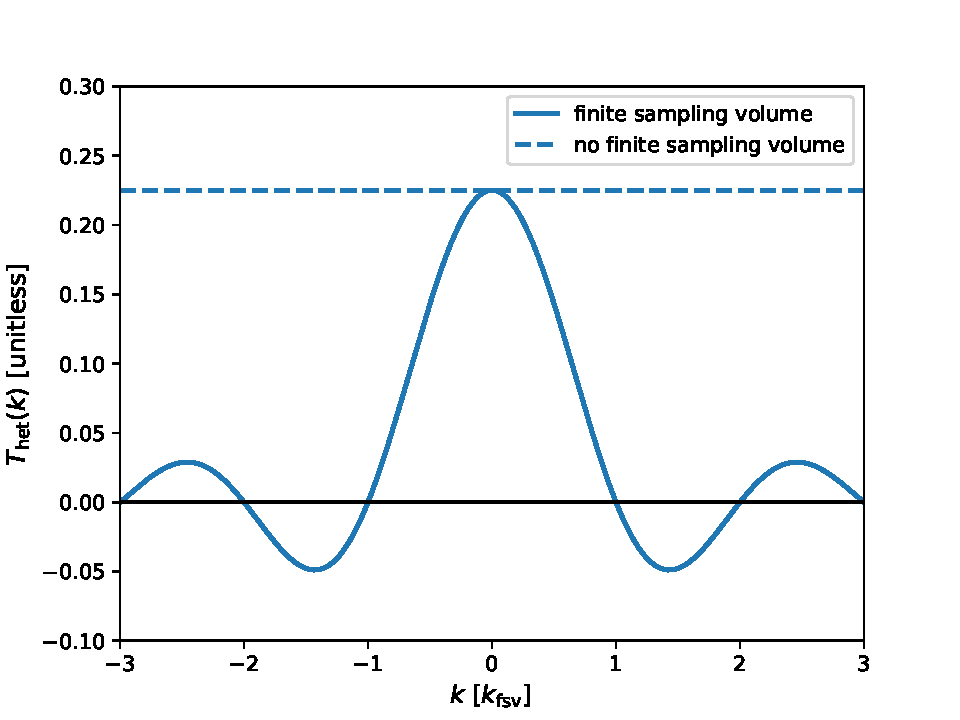
\includegraphics[width = \textwidth]{%
    Chapters/DesignConsiderations/figs/fsv_effects.pdf}
  \caption[Transfer function of heterodyne interferometer with finite sampling-volume effects]{%
    The wavenumber transfer function for a heterodyne interferometer
    with finite sampling-volume effects and
    without finite sampling-volume effects.
  }
\label{fig:DesignConsiderations:fsv_effects}
\end{figure}


\subsection{Depth of focus}
\label{sec:DesignConsiderations:geometric:depth_of_focus}
The derivations in
Sections~\ref{sec:InterferometricMethods:imaging} through
\ref{sec:InterferometricMethods:pci}
assumed that the detector sits exactly at the image plane.
Empirically, however, uncertainties in distances and focal lengths
produce a corresponding uncertainty in the image-plane location.
The axial distance by which the detector location may deviate
from the image plane is referred to as the \emph{depth of focus}.
Even if all components are perfectly positioned and
all focal lengths are equal to their nominal values,
the image plane still only maps to the tokamak midplane, and
images from points above and below the tokamak midplane
will be ``out of focus'';
such depth-of-field considerations are closely related
an imaging system's depth of focus.

In order to investigate a heterodyne interferometer's depth of focus,
it is necessary to generalize the derivation
of the imaged electric field from
Section~\ref{sec:InterferometricMethods:imaging}.
In particular, let the detector be located
an axial distance $\delta z_{\image}$ downstream of the image plane
(i.e.\ $z_{\text{det}} = z_{\image} + \delta z_{\image}$ such that
positive $\delta z_{\image}$ implies that
the detector is downstream of the image plane, and
negative $\delta z_{\image}$ implies that
the detector is upstream of the image plane).
Referencing the detector-plane coordinate transformation
(\ref{eq:ImagingSystems:coordinate_transformation_detector_plane}),
the imaged field at the detector
(\ref{eq:InterferometricMethods:imaged_total_field_monochromatic_fluctuation_weak_coupling})
readily generalizes to
\begin{equation}
  E(\vect{r}_{\text{det}}, t)
  \approx
  E_G(\vect{r}_{\text{det}}, t)
  e^{i \bar{\phi}}
  \left[%
    1
    +
    i e^{-i \mu} (\tilde{\phi}_0 \cos\nu')
  \right],
  \label{eq:DesignConsiderations:imaged_total_field_at_detector_plane}
\end{equation}
where
\begin{align}
  \mu
  &=
  \left( \frac{k_{\image}^2}{2 k_0} \right) \delta z_{\image},
  \\
  \nu'
  &=
  \left\{
    \left[ 1 - \frac{\delta z_{\image}}{R(z_{\text{det}})} \right]
    k_{\image}
  \right\}
  x_{\text{det}}
  -
  \omega t,
\end{align}
$k_{\image} = k / M$ is the image of wavenumber $k$
in a magnification-$M$ imaging system, and
$x_{\text{det}}$ and $\delta z_{\image}$ are assumed to be small
relative to the radius of curvature $R(z_{\text{det}})$
of the probe beam at the detector.
Relative to the image-plane field
(\ref{eq:InterferometricMethods:imaged_total_field_monochromatic_fluctuation_weak_coupling}),
the detector-plane field
(\ref{eq:DesignConsiderations:imaged_total_field_at_detector_plane})
has a wavenumber distortion
$\{1 - [\delta z_{\image} / R(z_{\text{det}})]\}$.
Additionally, the detector-plane field
has a wavenumber-dependent phase shift $\mu$, which
results from the ``out-of-focus'' interference of
the upscattered beam with the downscattered beam;
it has been empirically demonstrated that
blocking one of these scattered beams
eliminates this wavenumber-dependent phase shift
\cite[Sec.~2.1]{dorris_phd}, albeit at the expense
of reducing the amplitude of the fluctuating signal by a factor of two.

Heterodyne detection is implemented by interfering the detector-plane field
(\ref{eq:DesignConsiderations:imaged_total_field_at_detector_plane})
with a frequency-shifted reference beam.
In particular, assume a reference beam of the form
$E_G(\vect{r}_{\text{det}}, t) e^{-i \Delta \omega_0 t}$ such that
intensity (averaged over an optical cycle) becomes
\begin{equation}
  \begin{aligned}
    I_{\text{het}}(\vect{r}_{\text{det}}, t)
    =
    2 I_G(\vect{r}_{\text{det}})
    \bigl[%
      1
      &+
      \cos(\Delta \omega_0 t + \bar{\phi})
      \\
      &-
      \tilde{\phi}_0 \cos\nu'
      \sin(\Delta \omega_0 t + \bar{\phi} - \mu)
    \bigr].
  \end{aligned}
\end{equation}
Demodulating this heterodyne intensity via the program in
Section~\ref{sec:InterferometricMethods:interferometry},
one obtains the equilibrium and fluctuating components
of the in-phase and quadrature intensities
\begin{align}
  \bar{I}_{I}(\vect{r}_{\text{det}}, t)
  &=
  \frac{2 \sqrt{2}}{\pi}
  I_G(\vect{r}_{\text{det}}) \cos\bar{\phi},
  \\
  \bar{I}_{Q}(\vect{r}_{\text{det}}, t)
  &=
  \frac{2 \sqrt{2}}{\pi}
  I_G(\vect{r}_{\text{det}}) \sin\bar{\phi},
  \\
  \tilde{I}_{I}(\vect{r}_{\text{det}}, t)
  &=
  -\frac{2 \sqrt{2}}{\pi}
  I_G(\vect{r}_{\text{det}})
  \sin\left(\bar{\phi} - \mu\right)
  \cdot
  \tilde{\phi}_0 \cos\nu',
  \\
  \tilde{I}_{Q}(\vect{r}_{\text{det}}, t)
  &=
  \frac{2 \sqrt{2}}{\pi}
  I_G(\vect{r}_{\text{det}})
  \cos\left(\bar{\phi} - \mu\right)
  \cdot
  \tilde{\phi}_0 \cos\nu'.
\end{align}
It is possible to compute the autospectral density of the phase fluctuations
by summing the autospectral densities of $\tilde{I}_I$ and $\tilde{I}_Q$ and
then normalizing by $(\bar{I}_I^2 + \bar{I}_Q^2)$,
which fortuitously \emph{eliminates} the $\mu$-dependence.
However, it is \emph{not} readily apparent
how to extend this method to the computation of e.g.\
cross-spectral densities~\cite[Sec.~5.2]{bendat_and_piersol} and
bispectral densities~\cite{young_and_powers_ieee79},
for which the actual phase signal $\tilde{\phi}(x, t)$ is needed.
For this reason, the phase is often computed
via the inverse-tangent method discussed in
Section~\ref{sec:DesignConsiderations:demodulation:ideal}.
Unfortunately, this inverse-tangent method
has reduced response when $\mu \neq 0$.
To see this, first consider the case when $\mu = 0$:
$\bar{I}_I$ and $\bar{I}_Q$ map out a circle, and
the fluctuation $\tilde{\phi}_0 \cos\nu'$
produces perturbations $\tilde{I}_I$ and $\tilde{I}_Q$
that are always \emph{tangent} to this circle,
producing angular deviations in the $(I, Q)$-plane
that can be quantified by the inverse-tangent calculation.
Now, if $\mu \neq 0$, the perturbations $\tilde{I}_I$ and $\tilde{I}_Q$
are no longer tangent to the circle mapped out by $\bar{I}_I$ and $\bar{I}_Q$;
in the extreme that $\mu = (2m + 1) \pi / 2$ for integer $m$,
the fluctuations become purely \emph{radial} in the $(I, Q)$-plane, and
the inverse-tangent calculation, sensitive only to angular displacements,
fails to detect the fluctuations.


\section{Intensity considerations}
\label{sec:DesignConsiderations:intensity}
Ideally, a photovoltaic detector produces an output voltage
\begin{equation}
  V(t) = \mathcal{R}_0 \cdot I(t),
\end{equation}
where $\mathcal{R}_0$ is the detector responsivity and
$I(t)$ is the incident optical intensity.
However, every real-world detector has a saturation intensity $I_{\text{sat}}$
beyond which the output voltage ceases to be a linear function
of the incident optical intensity; that is,
the detector responsivity has an intensity dependence $\mathcal{R}(I)$, and
the detector voltage can be more generally written as
\begin{equation}
  V(t) = \mathcal{R}\left( I(t) \right) \cdot I(t).
\end{equation}
Here, $\mathcal{R}(I)$ is an arbitrary monotonically increasing function
of the incident optical intensity $I$.
Despite the potentially nonlinear response,
the detector voltage remains periodic in $2 \pi / \Delta \omega_0$ and
can be expanded in a Fourier series as
\begin{equation}
  V(t)
  =
  V_0
  +
  \sum_{n = 1}^{\infty}
  V_n \cos\left( n \Delta \omega_0 t + \theta_n \right),
\end{equation}
where $V_n$ and $\theta_n$ are the amplitude and phase, respectively,
of the $n\ts{th}$ harmonic.
Thus, a nonlinear detector response produces
higher-order harmonics in the signal.
In general, $V_n$ and $\theta_n$ can vary in time,
producing sidebands about each harmonic.
Provided the bandwidth of these fluctuations is sufficiently low,
there will be no spectral overlap
between the sidebands of adjacent harmonics, and
bandpass filtering the detector signal about $\Delta \omega_0$ yields
\begin{equation}
  V(t) \approx V_1 \cos[\Delta \omega_0 t + \theta_1(t)]
  \label{eq:DesignConsiderations:bandpass_filtered_voltage}
\end{equation}
with $\theta_1(t) = \phi(t)$, where
$\phi(t)$ is the optical phase shift
between the plasma and reference arms of the interferometer.
However, for fluctuations with sufficiently high bandwidth
(e.g.\ $\omega \sim \Delta\omega_0 / 2$),
the sidebands of adjacent harmonics begin to overlap,
potentially corrupting the phase measurement,
as demonstrated by the example in
Figure~\ref{fig:DesignConsiderations:nonlinear_heterodyne_detection}.
By processing the bandpass-filtered voltage
(\ref{eq:DesignConsiderations:bandpass_filtered_voltage})
via a procedure similar to that outlined between
(\ref{eq:InterferometricMethods:heterodyne_interferometer_I_and_Q_intensity})
and
(\ref{eq:InterferometricMethods:heterodyne_interferometer_wavenumber_transfer_function}),
one readily finds that
the heterodyne interferometer's wavenumber transfer function
(\ref{eq:InterferometricMethods:heterodyne_interferometer_wavenumber_transfer_function})
should be multiplied by the factor
$[V_1 / V_1(I_{\text{max}} = I_{\text{sat}})]$, where
$V_1$ is the amplitude of the bandpass-filtered voltage
(\ref{eq:DesignConsiderations:bandpass_filtered_voltage}), and
$V_1(I_{\text{max}} = I_{\text{sat}})$
is the amplitude of the corresponding bandpass-filtered voltage
when the system's maximum intensity is scaled to the saturation intensity
(the AC and DC fractions of the incident intensity
are \emph{not} altered during this scaling;
to account for changing the AC and DC fractions, see the discussion in
Section~\ref{sec:DesignConsiderations:geometric:beam_mismatch}).

\begin{figure}
  \centering
  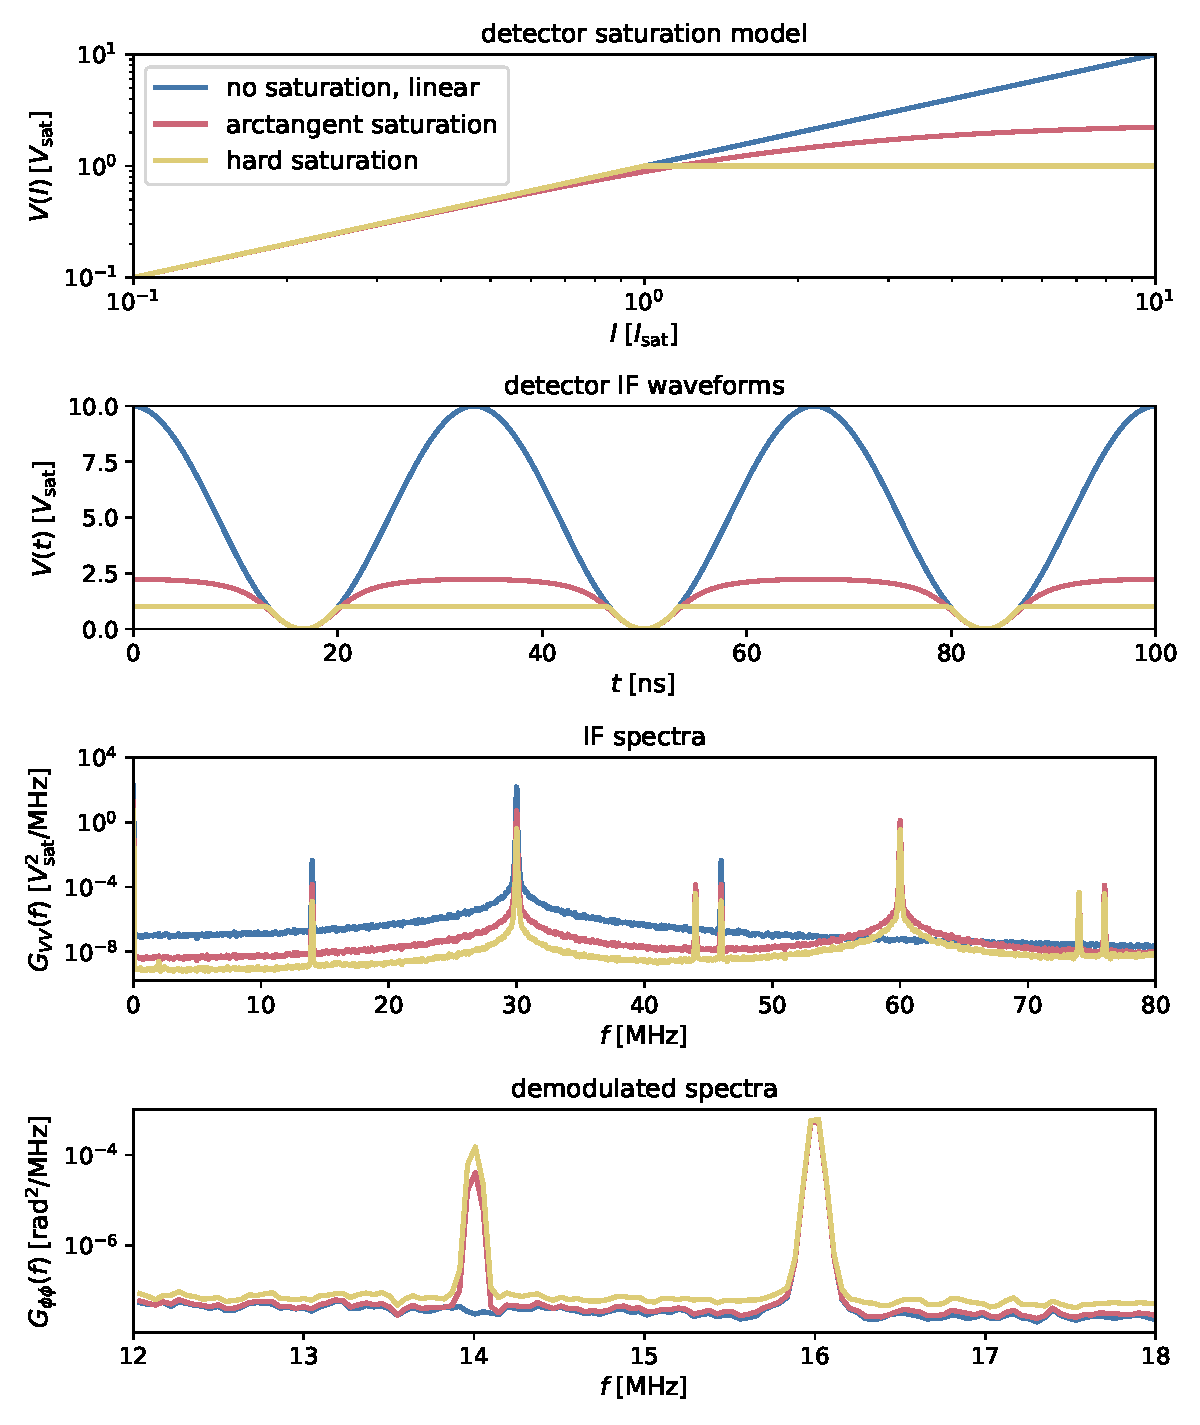
\includegraphics[width = \textwidth]{%
    Chapters/DesignConsiderations/figs/nonlinear_heterodyne_detection.pdf}
  \caption[Heterodyne detection beyond the saturation intensity]{%
    Heterodyne detection beyond the saturation intensity with
    $\Delta\omega_0 = 2\pi \cdot \SI{30}{\mega\hertz}$ and
    $\omega = 2 \pi \cdot \SI{16}{\mega\hertz}$.
    (Top panel): Various detector saturation models.
    The linear model exhibits no saturation,
    the hard saturation model limits the output voltage
    to $V_{\text{sat}}$ when the incident optical intensity
    exceeds $I_{\text{sat}}$, and
    the arctangent saturation model exhibits $\SI{1}{\deci\bel}$ compression
    when the incident optical intensity is $I_{\text{sat}}$.
    (2\ts{nd} panel): The intermediate frequency (IF) waveforms
    corresponding to each saturation model when
    $I_{\text{max}} = 10 \, I_{\text{sat}}$.
    The arctangent and hard saturation models distort the IF waveform,
    producing numerous higher-order harmonics.
    (3\ts{rd} panel): Autospectral densities of the IF waveforms.
    The IF waveforms all exhibit peaks at
    the $\SI{30}{\mega\hertz}$ fundamental and
    its corresponding sidebands at
    $\SI{30}{\mega\hertz} \pm \SI{16}{\mega\hertz}$.
    However, the saturated IF waveforms
    also exhibit peaks at the second harmonic ($\SI{60}{\mega\hertz}$)
    and its corresponding sidebands
    ($\SI{60}{\mega\hertz} \pm \SI{16}{\mega\hertz}$).
    (Bottom panel): Autospectral densities of the demodulated phase.
    Note that the $\SI{16}{\mega\hertz}$ fluctuation is correctly identified
    when demodulating all of the IF waveforms.
    However, the saturated IF waveforms also produce
    a \emph{spurious} $\SI{14}{\mega\hertz}$ fluctuation,
    which is attributable to the overlap of
    the $\SI{30}{\mega\hertz}$ and $\SI{60}{\mega\hertz}$ sidebands.
  }
\label{fig:DesignConsiderations:nonlinear_heterodyne_detection}
\end{figure}


\section{Phase noise: sources \& effects}
\label{sec:DesignConsiderations:phase_noise}
Heterodyne interferometry at $\SI{10.6}{\micro\meter}$ relies on both
an optical oscillator (the laser) and
a radio-frequency oscillator
(usually referred to as the local oscillator (LO)).
These oscillators, like all real-world oscillators, exhibit phase noise.
The spectral properties and implications of oscillator phase noise
are reviewed in Appendix~\ref{app:OscillatorPhaseNoise}.
Below, Section~\ref{sec:DesignConsiderations:phase_noise:laser}
shows that a mismatch between the optical path lengths
of the probe beam and the reference beam
injects the laser's phase noise
into the heterodyne interferometer's measurements, while
Section~\ref{sec:DesignConsiderations:phase_noise:LO}
shows that finite coupling time
in the Doppler-shifting modulator
injects the LO's phase noise
into the heterodyne interferometer's measurements.


\subsection{Unmatched optical path lengths \& laser phase noise}
\label{sec:DesignConsiderations:phase_noise:laser}
The external reference-beam interferometry derivations
in Section~\ref{sec:InterferometricMethods:interferometry}
assumed that the laser's angular frequency was fixed
at its nominal value $\omega_0$.
However, the angular frequency of any \emph{real} laser
will exhibit small fluctuations in time,
much like any other real-world oscillator
\cite[Sec.~1.7]{siegman_lasers}.
The electric field of such a Gaussian beam
is well-described by
\begin{equation}
  E_G(\vect{r}, t)
  =
  E_G(\vect{r})
  e^{-i [\omega_0 t + \phi_{\omega_0}(t)]},
\end{equation}
where $\phi_{\omega_0}(t)$ is a zero-mean, stationary, random process
known as the laser's \emph{phase deviation}
whose temporal variation causes
the laser's instantaneous angular frequency
to wander about its nominal value $\omega_0$.

Now, if the interferometer's probe beam and reference beam
traverse different optical path lengths,
the laser's phase deviation will inject
phase noise into the measured signal.
To see this, assume that the optical path length of the probe beam
exceeds that of the reference arm by $L$.
Then, if the reference beam impinging on the detector at time $t$ is
\begin{equation}
  E_R(\vect{r}_{\image}, t)
  =
  E_G(\vect{r}_{\image})
  e^{-i [
    (\omega_0 + \Delta \omega_0) t
    +
    \phi_{\omega_0}(t)
  ]},
\end{equation}
the corresponding imaged probe radiation from
(\ref{eq:InterferometricMethods:imaged_total_field_interferometer})
becomes
\begin{equation}
  E_P(\vect{r}_{\image}, t)
  =
  E_G(\vect{r}_{\image})
  e^{-i [\omega_0 (t - \tau) + \phi_{\omega_0}(t - \tau)]}
  e^{i \bar{\phi}}
  \left[%
    1
    +
    i \tilde{\phi}(x_{\image}, t)
  \right],
\end{equation}
where $\tau = L / c$ is the time delay
associated with the optical path-length difference $L$.
The resulting intensity (averaged over an optical cycle)
of the interfering radiation is
\begin{equation}
  \begin{aligned}
    I_{\text{het}}(\vect{r}_{\image}, t)
    \approx
    2 I_G(\vect{r}_{\image})
    \bigl[%
      1
      &+
      \cos(\Delta \omega_0 t + \bar{\phi}_{\text{eff}})
      \\
      &-
      \tilde{\phi}_m(x_{\image}, t)
      \sin(\Delta \omega_0 t + \bar{\phi}_{\text{eff}})
    \bigr],
  \end{aligned}
  \label{eq:DesignConsiderations:heterodyne_intensity_with_laser_phase_noise}
\end{equation}
where
\begin{align}
  \bar{\phi}_{\text{eff}}
  &=
  \bar{\phi} + \omega_0 \tau,
  \\
  \tilde{\phi}_m(x_{\image}, t)
  &=
  \tilde{\phi}(x_{\image}, t) + \delta \phi_{\omega_0}(t - \tau, \tau),
  \label{eq:DesignConsiderations:measured_phase_with_laser_phase_noise}
  \\
  \delta \phi_{\omega_0}(t, \tau)
  &=
  \phi_{\omega_0}(t + \tau)
  -
  \phi_{\omega_0}(t).
\end{align}
The quantity $\delta \phi_{\omega_0}(t, \tau)$
is referred to as the ``instrumental phase noise'', and
it is produced by the optical path-length difference $L$ and
the laser's phase deviation $\phi_{\omega_0}(t)$.
Typically, $|\delta \phi_{\omega_0}(t, \tau)| \ll 1$, and
only terms to first order in $\delta \phi_{\omega_0}$ and $\tilde{\phi}$
were retained in the heterodyne intensity
(\ref{eq:DesignConsiderations:heterodyne_intensity_with_laser_phase_noise}).
Comparing
(\ref{eq:DesignConsiderations:heterodyne_intensity_with_laser_phase_noise})
with (\ref{eq:InterferometricMethods:heterodyne_intensity}),
one readily sees that
the \emph{measured} phase fluctuation is $\tilde{\phi}_m$ defined in
(\ref{eq:DesignConsiderations:measured_phase_with_laser_phase_noise});
that is, the fluctuating signal is contaminated
by the instrumental phase noise.
The spectral properties of $\delta \phi_{\omega_0}(t, \tau)$
are thoroughly discussed in Appendix~\ref{app:OscillatorPhaseNoise}.
As $\delta \phi_{\omega_0}(t, \tau)$ and
$\tilde{\phi}(x_{\image}, t)$ are uncorrelated,
the one-sided autospectral density of the measured phase fluctuations is
\begin{equation}
    G_{\tilde{\phi}_m,\tilde{\phi}_m}(f)
    =
    G_{\tilde{\phi},\tilde{\phi}}(f)
    +
    8 \sin^2(\pi f \tau) \mathcal{L}_{\omega_0}(f),
\end{equation}
where
$G_{\tilde{\phi},\tilde{\phi}}(f)$ is the \emph{true}
one-sided autospectral density of the phase fluctuation $\tilde{\phi}$ and
$\mathcal{L}_{\omega_0}(f)$ is the phase noise of the laser,
as defined in Appendix~\ref{app:OscillatorPhaseNoise}.


\subsection{Modulator's finite coupling time \& LO phase noise}
\label{sec:DesignConsiderations:phase_noise:LO}
Heterodyne detection is effected by
modestly Doppler shifting the reference beam
relative to the plasma beam.
It is easy to Doppler shift $\SI{10.6}{\micro\meter}$ radiation
by tens of $MHz$ with a Germanium acousto-optic modulator (AOM).
The operation of a typical AOM is sketched in
Figure~\ref{fig:DesignConsiderations:aom_scattering_diagram}.
A piezo-actuator drives sound waves
of angular frequency $\Delta \omega_0$
through the Germanium crystal, and
the sound waves act as a diffraction grating
that propagates at the crystal's sound speed $c_s$.
When a beam of vacuum wavelength $\lambda_0$
impinges upon the crystal at the Bragg angle
\begin{equation}
  \theta_B = \frac{\lambda_0 \cdot \Delta \omega_0}{4 \pi c_s},
  \label{eq:DesignConsiderations:Bragg_angle}
\end{equation}
a portion of the beam is deflected and
Doppler shifted by angular frequency $\Delta \omega_0$
\cite[Sec.~20.1]{saleh_and_teich}.
The power in the deflected beam
is controlled by the intensity of the sound waves.

\begin{figure}
  \centering
  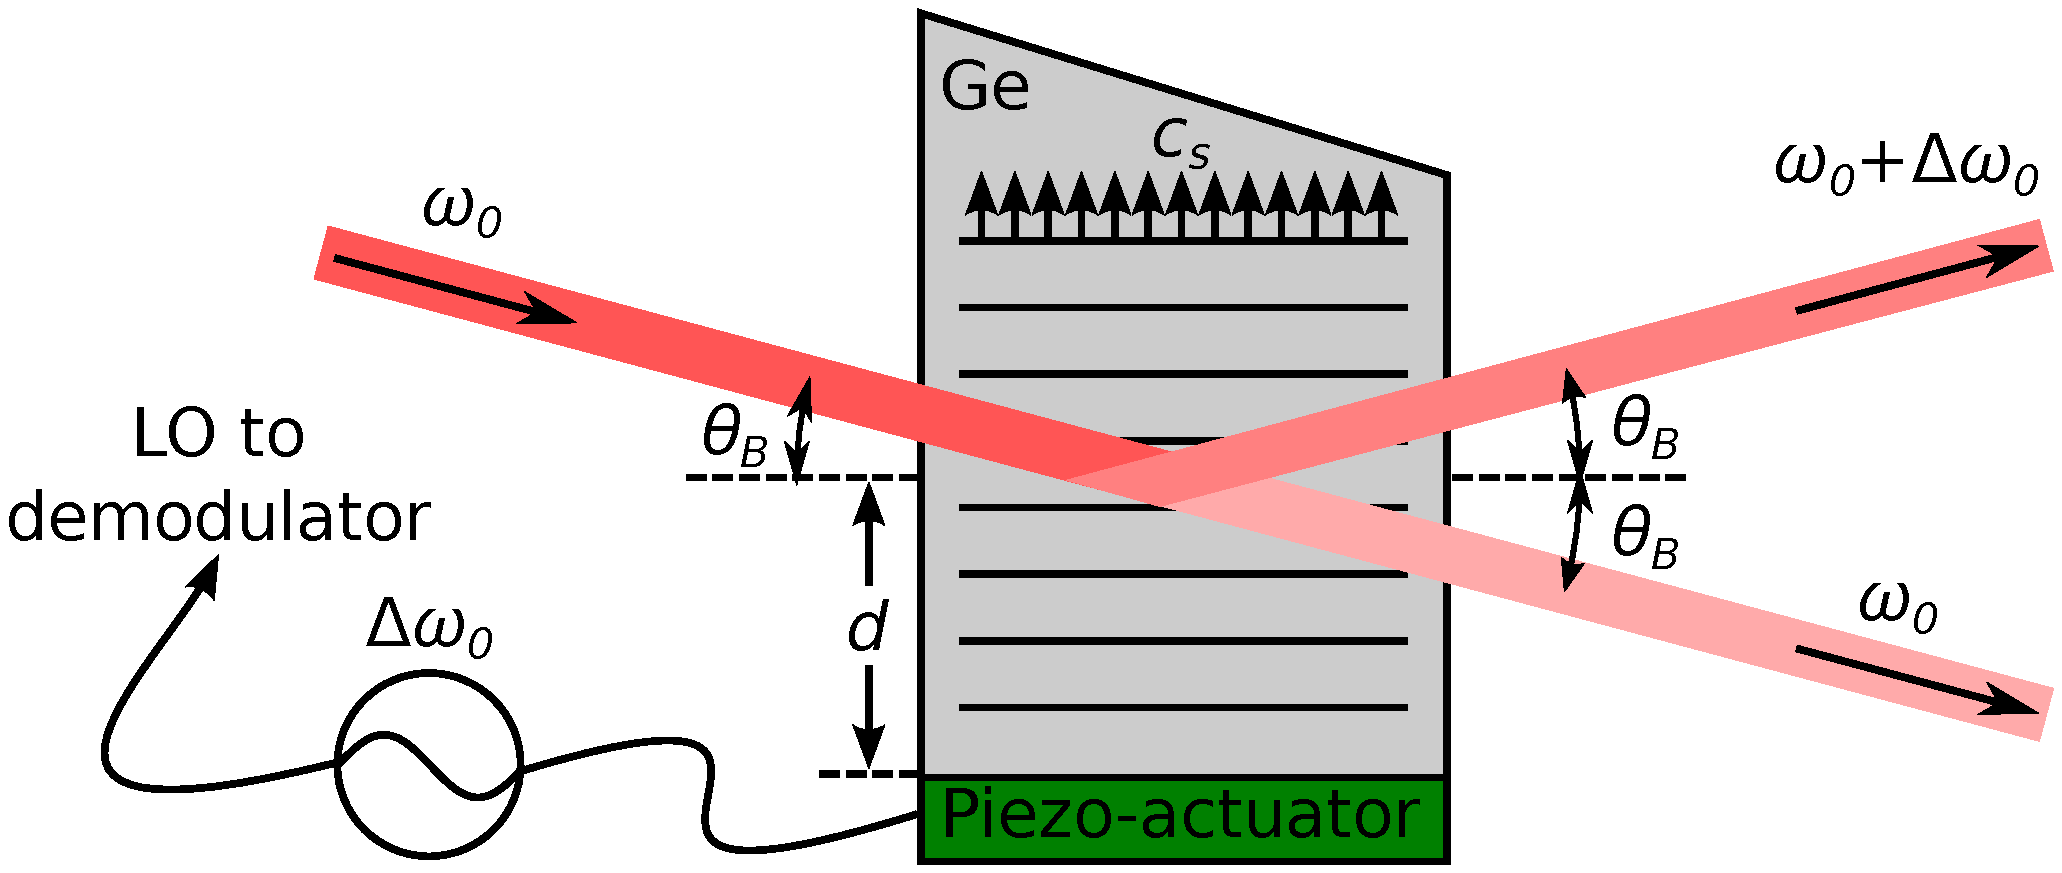
\includegraphics[width = \textwidth]{%
    Chapters/DesignConsiderations/figs/aom_scattering_diagram.pdf}
  \caption[Illustration of AOM operation in a heterodyne interferometer]{%
    An illustration of AOM operation in a heterodyne interferometer.
    A piezo-actuator drives sound waves of angular frequency $\Delta \omega_0$
    through a crystal (usually Germanium for $\SI{10.6}{\micro\meter}$ light),
    and these sound waves deflect and Doppler shift light
    that is incident upon the crystal at the Bragg angle $\theta_B$.
    The sound waves propagate from the piezo-actuator
    to the AOM's optically active region
    over finite time $\tau = d / c_s$.
    The RF waveform that drives the piezo-actuator
    is sampled and used to demodulate the heterodyne interference signal.
    Note that for simplicity the refraction of the beam
    as it enters and exits the crystal is \emph{not} depicted.}
\label{fig:DesignConsiderations:aom_scattering_diagram}
\end{figure}

The coupling of the AOM's drive signal to the deflected beam
occurs on the crystal's sound-wave timescale.
If the sound waves must propagate a distance $d$
from the piezo-actuator to the AOM's optically active region,
the drive signal is coupled to the deflected beam
only after time delay $\tau = d / c_s$.
The sound speed in Germanium is $c_s = \SI{5400}{\meter\per\second}$
such that a distance $d = \SI{1}{\centi\meter}$
is accompanied by a time delay $\tau = \SI{1.85}{\micro\second}$.
Note that this is large compared to many other timescales
typically considered in interferometry;
for example, light propagates
through $\SI{1}{\meter}$ of air
in only $\SI{3.33}{\nano\second}$,
and an RF signal propagates
through $\SI{1}{\meter}$ of RG-58 coaxial cable
(for which the index of refraction is $\sim 3 / 2$)
in only $\SI{5}{\nano\second}$.

In the presence of LO phase noise,
an AOM's finite coupling time
can degrade the performance of a heterodyne interferometer.
A local oscillator with phase noise is well-described by
\begin{equation}
  V_{\text{LO}}(t)
  =
  V_{0}
  e^{-i [\Delta \omega_0 t + \phi_{\Delta \omega_0}(t)]},
\end{equation}
where $\phi_{\Delta \omega_0}(t)$ is a zero-mean, stationary, random process
known as the LO's \emph{phase deviation}
whose temporal variation causes
the LO's instantaneous angular frequency
to wander about its nominal value $\Delta \omega_0$.
Then, to account for the AOM's finite coupling time and
the LO phase noise, take
$\Delta \omega_0 t
\rightarrow
[\Delta \omega_0 (t - \tau) + \phi_{\Delta \omega_0}(t - \tau)]$
in the heterodyne intensity
(\ref{eq:InterferometricMethods:heterodyne_intensity}).
Neglecting finite sampling-volume effects,
the heterodyne output voltage from a given detector element
is simply proportional to the local intensity, i.e.\
\begin{align}
  \begin{aligned}
    V_{\text{het}}(t)
    &=
    2 V_0
    \bigl\{%
      1
      +
      \cos\left[%
        \Delta \omega_0 t
        +
        \bar{\phi}_{\text{eff}}
        +
        \phi_{\Delta \omega_0}(t - \tau)
      \right]
      \\
      &\quad-
      \tilde{\phi}(x_{\image}, t)
      \sin\left[%
        \Delta \omega_0 t
        +
        \bar{\phi}_{\text{eff}}
        +
        \phi_{\Delta \omega_0}(t - \tau)
      \right]
    \bigr\},
  \end{aligned}
\end{align}
where $\bar{\phi}_{\text{eff}} = \bar{\phi} - \Delta \omega_0 \tau$.
Then, taking inspiration from the demodulated optical intensities
(\ref{eq:InterferometricMethods:heterodyne_interferometer_I_and_Q_intensity}),
the demodulated in-phase ($V_I$) and quadrature ($V_Q$) voltages are defined as
\begin{align}
  V_{I}(t)
  +
  i \cdot V_{Q}(t)
  &=
  \frac{1}{V_0}
  \langle
    V_{\text{LO}}(t)
    \cdot
    V_{\text{het}}(t)
  \rangle_{\Delta \omega_0}
  \notag \\
  &=
  V_0
  e^{i \bar{\phi}_{\text{eff}}}
  \left[
    1
    +
    i \tilde{\phi}_m(x_{\image}, t)
  \right],
  \label{eq:DesignConsiderations:heterodyne_interferometer_I_and_Q_voltage}
\end{align}
where
\begin{align}
  \tilde{\phi}_m(x_{\image}, t)
  &=
  \tilde{\phi}(x_{\image}, t)
  +
  \delta \phi_{\Delta \omega_0}(t, -\tau),
  \label{eq:DesignConsiderations:measured_phase_with_LO_phase_noise}
  \\
  \delta \phi_{\Delta \omega_0}(t, \tau)
  &=
  \phi_{\Delta \omega_0}(t + \tau)
  -
  \phi_{\Delta \omega_0}(t).
\end{align}
The quantity $\delta \phi_{\Delta \omega_0}(t, \tau)$
is referred to as the ``instrumental phase noise'', and
it is produced by the modulator's finite coupling time $\tau$ and
the LO's phase deviation $\phi_{\Delta \omega_0}(t)$.
Typically, $|\delta \phi_{\Delta \omega_0}(t, \tau)| \ll 1$, and
only terms to first order in $\delta \phi_{\omega_0}$ and $\tilde{\phi}$
were retained in the demodulated voltages
(\ref{eq:DesignConsiderations:heterodyne_interferometer_I_and_Q_voltage}).
Comparing
(\ref{eq:DesignConsiderations:heterodyne_interferometer_I_and_Q_voltage})
with the demodulated intensities
(\ref{eq:InterferometricMethods:heterodyne_interferometer_I_and_Q_intensity}),
one readily sees that
the \emph{measured} phase fluctuation is $\tilde{\phi}_m$ defined in
(\ref{eq:DesignConsiderations:measured_phase_with_LO_phase_noise});
that is, the fluctuating signal is contaminated
by the instrumental phase noise.
The spectral properties of $\delta \phi_{\Delta\omega_0}(t, \tau)$
are thoroughly discussed in Appendix~\ref{app:OscillatorPhaseNoise}.
As $\delta \phi_{\omega_0}(t, \tau)$ and
$\tilde{\phi}(x_{\image}, t)$ are uncorrelated,
the one-sided autospectral density of the measured phase fluctuations is
\begin{equation}
    G_{\tilde{\phi}_m,\tilde{\phi}_m}(f)
    =
    G_{\tilde{\phi},\tilde{\phi}}(f)
    +
    8 \sin^2(\pi f \tau) \mathcal{L}_{\Delta\omega_0}(f),
\end{equation}
where
$G_{\tilde{\phi},\tilde{\phi}}(f)$ is the \emph{true}
one-sided autospectral density of the phase fluctuation $\tilde{\phi}$ and
$\mathcal{L}_{\Delta\omega_0}(f)$ is the phase noise of the LO,
as defined in Appendix~\ref{app:OscillatorPhaseNoise}.


\section{Amplitude noise: sources \& effects}
\label{sec:DesignConsiderations:amplitude_noise}
Detector noise and optical shot noise are
omnipresent contributors to amplitude noise
in the heterodyne interference signal, while
a noisy amplifier can degrade the signal-to-noise ratio.
The demodulation of such amplitude noise
is throughly discussed by Rakhmanov in~\cite{rakhmanov_ao01}.
While Rakhmanov does not explicitly consider quadrature heterodyne detection,
his results can be naturally applied to quadrature heterodyne detection,
as is done below.


\subsection{Detector noise}
\label{sec:DesignConsiderations:amplitude_noise:detector}
Real-world detector operation is associated with intrinsic noise.
This noise results from, among other things,
Johnson thermal noise in the detector and
shot noise in the background radiation flux
\cite{hamamatsu_ir_detectors}.
A detector's noise is often characterized by
its noise-equivalent power ($NEP$):
when the power of the incident optical signal is equal to the $NEP$,
the signal-to-noise ratio is unity.
Consider optical power $\delta P(t)$ that, when incident upon a detector,
produces a signal that
emulates the statistical properties of the detector noise
(e.g.\ $\delta P(t)$ is a real-valued, zero-mean, stationary, random process).
Then, the $NEP$ corresponds to the root mean square (RMS) of $\delta P(t)$,
and
\begin{equation}
  (NEP)^2
  =
  \int_{\Delta f}
  G_{\delta P, \delta P}(f) df,
  \label{eq:DesignConsiderations:NEP_from_spectral_density}
\end{equation}
where $G_{\delta P, \delta P}(f)$ is
the one-sided autospectral density of $\delta P(t)$ and
the integral is performed over the temporal bandwidth $\Delta f$
of the desired measurement.
Note that $G_{\delta P, \delta P}(f)$ depends on both
extensive (e.g.\ element area) and intensive (e.g.\ element material)
properties of the detector.
To more easily compare detectors of different sizes and materials,
the $NEP$ of a given detector is often parameterized as
\begin{equation}
  NEP = \frac{\sqrt{A \cdot \Delta f}}{D^{*}},
  \label{eq:DesignConsiderations:NEP_from_engineering_parameters}
\end{equation}
where $A$ is the effective area of the detector element,
$\Delta f$ is the temporal bandwidth of the desired measurement, and
$D^{*}$ is the detector's specific detectivity~\cite{jones_josa60}.
Note that larger $D^{*}$ corresponds to increased detector sensitivity.
If $G_{\delta P, \delta P}(f)$ is approximately constant
over the bandwidth $\Delta f$, then equating
(\ref{eq:DesignConsiderations:NEP_from_spectral_density})
to the square of
(\ref{eq:DesignConsiderations:NEP_from_engineering_parameters})
yields
\begin{equation}
  G_{\delta P, \delta P}(f)
  =
  \frac{A}{(D^*)^2}.
  \label{eq:DesignConsiderations:NEP_spectral_density}
\end{equation}

It is now shown shown that
signal demodulation pushes detector noise
near the heterodyne angular frequency $\Delta \omega_0$
into the baseband signal.
Taking inspiration from the demodulated optical intensities
(\ref{eq:InterferometricMethods:heterodyne_interferometer_I_and_Q_intensity}),
define the total $NEP$ contamination of
the in-phase ($I$) and quadrature ($Q$) signals to be
\begin{align}
  \delta P_{IQ}(t)
  =
  \frac{2 \sqrt{2}}{\pi}
  e^{- i \Delta \omega_0 t} \cdot \delta P(t).
  \label{eq:DesignConsiderations:demodulated_NEP_complex}
\end{align}
Here, the demodulated noise has \emph{not} yet been low-pass filtered.
The autocorrelation function of the demodulated noise is
\begin{align}
  R_{\delta P_{IQ},\delta P_{IQ}}(\tau)
  &=
  E\left[\delta P_{IQ}(t) \cdot \delta P_{IQ}^*(t + \tau) \right]
  \notag \\
  &=
  \frac{8}{\pi^2}
  \cdot
  e^{i \Delta \omega_0 \tau}
  \cdot
  R_{\delta P, \delta P}(\tau),
\end{align}
where $z^*$ indicates the complex conjugate of $z$ and
$R_{\delta P, \delta P}(\tau)$ is the
autocorrelation function of the $NEP$.
The autospectral density of the demodulated noise is then
\begin{align}
  S_{\delta P_{IQ},\delta P_{IQ}}(f)
  &=
  \mathcal{F}\left[ R_{\delta P_{IQ},\delta P_{IQ}}(\tau) \right](f)
  \notag \\
  &=
  \frac{8}{\pi^2}
  \cdot
  \mathcal{F}\left[
    e^{i 2 \pi \Delta f_0 \tau} \cdot R_{\delta P, \delta P}(\tau)
  \right](f)
  \notag \\
  &=
  \frac{8}{\pi^2}
  \cdot
  S_{\delta P, \delta P}(f + \Delta f_0),
\end{align}
where
$\Delta f_0 = \Delta \omega_0 / (2 \pi)$ is the heterodyne frequency and
$S_{\delta P, \delta P}(f)$ is the autospectral density of the $NEP$.
The demodulated signals are typically low-pass filtered
such that only the desired information at $|f| \ll \Delta f_0$
survives
\begin{equation}
  \left.
    S_{\delta P_{IQ},\delta P_{IQ}}(f)
  \right|_{|f| \ll \Delta f_0}
  \approx
  \frac{8}{\pi^2}
  \cdot
  S_{\delta P, \delta P}(\Delta f_0).
  \label{eq:DesignConsiderations:detector_noise_demodulated}
\end{equation}
Thus, the $NEP$ at the heterodyne frequency $\Delta f_0$
is pushed into the baseband signal via the demodulation process.
Note that the autospectral density of the demodulated detector noise
(\ref{eq:DesignConsiderations:detector_noise_demodulated})
is in agreement with the literature
(e.g.\ see Rakhmanov's Eq.~(47) in~\cite{rakhmanov_ao01}
with $d_1 = 2 / \pi$ for demodulation against
the \emph{first harmonic} of a zero-mean square wave
with frequency $\Delta f_0$ and peak-to-peak amplitude of two;
see Section~\ref{sec:DesignConsiderations:demodulation:nonideal_mixing}
for the physical significance of demodulation against such a square wave).
The corresponding one-sided autospectral density
of the demodulated detector noise is
\begin{align}
  \left.
    G_{\delta P_{IQ},\delta P_{IQ}}(f)
  \right|_{|f| \ll \Delta f_0}
  &\approx
  \frac{8}{\pi^2}
  \cdot
  G_{\delta P, \delta P}(\Delta f_0).
  \notag \\
  &=
  \frac{8}{\pi^2}
  \cdot
  \frac{A}{(D^*)^2},
  \label{eq:DesignConsiderations:demodulated_NEP_spectral_density}
\end{align}
where the last line follows from
(\ref{eq:DesignConsiderations:NEP_spectral_density}) and
the assumption that $D^{*}$ is the specific detectivity
for frequencies $f$ in the neighborhood
of the heterodyne frequency $\Delta f_0$.

Note that comparing the spectral density
of the demodulated detector noise
to the spectral density of the measured phase
(with the phase having units of radians)
requires converting
(\ref{eq:DesignConsiderations:demodulated_NEP_spectral_density})
from units of $\SI{}{\watt\squared\per\Hz}$
to the corresponding angular equivalent.
This unit conversion is accomplished by dividing
(\ref{eq:DesignConsiderations:demodulated_NEP_spectral_density})
by the \emph{square} of the total demodulated power in the $I$ and $Q$ signals.
Assuming that the probe beam and the reference beam
vary weakly over the face of the detector element,
this squared power is
$P_{IQ}^2 \approx (8 / \pi^2) P_P P_R$, where
$P_P$ is the optical power of the probe beam impinging on the detector, and
$P_R$ is the optical power of the reference beam impinging on the detector.
Thus, the one-sided autospectral density of the demodulated detector noise
(in angular units of $\SI{}{\radian\squared\per\Hz}$) is
\begin{equation}
  \left.
    G_{\delta P_{IQ},\delta P_{IQ}}(f)
  \right|_{|f| \ll \Delta f_0}
  =
  \frac{A}{P_P P_R (D^*)^2}.
\end{equation}


\subsection{Optical shot noise}
\label{sec:DesignConsiderations:amplitude_noise:shot}
The discrete nature of the arriving photons results in shot noise.
Well-modeled as a Poisson process,
the optical shot noise increases as $N_{\gamma}^{1/2}$, where
$N_{\gamma}$ is the number of incident photons.
Because the incident optical power (and hence the number of incident photons)
in the heterodyne optical signal is modulated as a function of time,
the corresponding shot noise is inherently nonstationary.
Surprisingly, however, the demodulated shot noise \emph{is} stationary
(e.g.\ see Rakhmanov's Eq.~(59) in~\cite{rakhmanov_ao01}).
Note that Rakhmanov only considers \emph{one} of the demodulated signals, and
maximizing the signal-to-noise ratio in the demodulated signal
requires careful selection of the local oscillator's phase
relative to that of the heterodyne signal
(he terms this the ``demodulation phase'' and
represents it via $\gamma$).
However, by employing quadrature heterodyne detection~\cite{carlstrom_rsi88},
in which $\gamma_Q = \gamma_I + \pi / 2$,
the total shot-noise contamination $\delta P_{IQ}$
of the in-phase ($I$) and quadrature ($Q$) signals
(with $\delta P_{IQ}$ as defined in
(\ref{eq:DesignConsiderations:demodulated_NEP_complex}),
but with $\delta P$ now corresponding to the shot-noise optical power)
is \emph{independent} of the demodulation phase, i.e.\
\begin{align}
  \left.
    S_{\delta P_{IQ}, \delta P_{IQ}}(f)
  \right|_{|f| \ll \Delta f_0}
  &=
  \frac{8}{\pi^2}
  \cdot
  h f_0 P_0,
\end{align}
where
$h$ is the Planck constant,
$f_0$ is the frequency of the incident photons, and
$P_0$ is the DC optical power impinging upon the detector.
The corresponding one-sided autospectral density is
\begin{align}
  \left.
    G_{\delta P_{IQ}, \delta P_{IQ}}(f)
  \right|_{|f| \ll \Delta f_0}
  =
  \frac{16}{\pi^2}
  \cdot
  h f_0 P_0.
  \label{eq:DesignConsiderations:demodulated_shot_noise_spectral_density}
\end{align}
Rakhmanov notes that
(\ref{eq:DesignConsiderations:demodulated_shot_noise_spectral_density})
corresponds to the well-known Schottky formula.

Note that comparing the spectral density
of the demodulated optical shot noise
to the spectral density of the measured phase
(with the phase having units of radians)
requires converting
(\ref{eq:DesignConsiderations:demodulated_shot_noise_spectral_density})
from units of $\SI{}{\watt\squared\per\Hz}$
to the corresponding angular equivalent.
This unit conversion is accomplished by dividing
(\ref{eq:DesignConsiderations:demodulated_NEP_spectral_density})
by the \emph{square} of the total demodulated power in the $I$ and $Q$ signals.
Assuming that the probe beam and the reference beam
vary weakly over the face of the detector element,
this squared power is
$P_{IQ}^2 \approx (8 / \pi^2) P_P P_R$, where
$P_P$ is the optical power of the probe beam impinging on the detector, and
$P_R$ is the optical power of the reference beam impinging on the detector.
Additionally, the DC optical power impinging upon the detector is
$P_0 = P_P + P_R$.
Thus, the one-sided autospectral density
of the demodulated optical shot noise
(in angular units of $\SI{}{\radian\squared\per\Hz}$) is
\begin{equation}
  \left.
    G_{\delta P_{IQ}, \delta P_{IQ}}(f)
  \right|_{|f| \ll \Delta f_0}
  =
  2 h f_0 \left( \frac{P_P + P_R}{P_P P_R} \right).
\end{equation}


\subsection{Amplifier noise}
\label{sec:DesignConsiderations:amplitude_noise:amplifier}
The noise \emph{factor} $F$ of an RF amplifier is defined as the ratio of
the signal-to-noise ratio at the device's input ($SNR_{\text{in}}$) to
the signal-to-noise ratio at the device's output ($SNR_{\text{out}}$)
\begin{equation}
  F = \frac{SNR_{\text{in}}}{SNR_{\text{out}}};
\end{equation}
often, the noise factor $F$ is given
in terms of the noise \emph{figure} $NF$
\cite{minicircuits_amplifier_terms_defined}
\begin{equation}
  NF = 10 \log_{10} F.
\end{equation}
If several amplifiers are cascaded,
the total noise factor of the amplifier chain
can be computed using the well-known Friis noise-factor formula.
Note that the noise factor is only defined
in the context of a signal-to-noise ratio, so
it is not conventional to write down the corresponding
autospectral density of the amplifier noise in absolute units.


\section{Demodulation}
\label{sec:DesignConsiderations:demodulation}
The heterodyne interferometer's intermediate frequency (IF) signal
must be demodulated in order to recover the baseband phase information.
Demodulation is typically described as an analog process
in which the IF signal is \emph{mixed} with a local oscillator (LO), but
demodulation can also be performed digitally
\cite{vanzeeland_rsi08, mlynek_fst12} or
with non-mixer-based analog electronics~\cite{mlynek_rsi17}.
The focus here, however, is on the analog, mixer-based approach.
Section~\ref{sec:DesignConsiderations:demodulation:ideal}
describes ideal analog demodulation.
Sections~\ref{sec:DesignConsiderations:demodulation:nonideal_mixing} and
\ref{sec:DesignConsiderations:demodulation:demodulator_imbalances}
discuss nonideal aspects of analog mixers and demodulators, and
Section~\ref{sec:DesignConsiderations:demodulation:imperfection_implications}
analyzes the implications of these imperfections
in the context of fluctuation measurements.


\subsection{Ideal demodulation}
\label{sec:DesignConsiderations:demodulation:ideal}
A typical analog $I\&Q$ demodulator consists of
a $90^{\circ}$ splitter,
two double-balanced mixers, and
a $0^{\circ}$ splitter~\cite{minicircuits_modulators}, as shown in
Figure~\ref{fig:DesignConsiderations:analog_IQ_demodulator}(a).
The $90^{\circ}$ splitter divides the incident local oscillator (LO) signal
\begin{equation}
  \text{LO}(t) = \frac{4 \sqrt{2}}{\pi} \cos(\Delta\omega_0 t)
\end{equation}
into an ``in-phase'' copy of the LO
\begin{equation}
  \text{LO}_0(t)
  =
  \frac{4}{\pi} \cos(\Delta\omega_0 t)
\end{equation}
and a $\pi / 2$ phase-advanced copy of the LO
\begin{equation}
  \text{LO}_{\pi / 2}(t)
  =
  \frac{4}{\pi} \cos\left( \Delta\omega_0 t + \frac{\pi}{2} \right)
  =
  -\frac{4}{\pi} \sin(\Delta\omega_0 t).
\end{equation}
Note that the power (i.e.\ the mean-square value) in the incident LO signal
is split evenly between $\text{LO}_0(t)$ and $\text{LO}_{\pi / 2}(t)$.
Further, the normalization of $\text{LO}_0(t)$ and $\text{LO}_{\pi / 2}(t)$
is motivated by and is consistent with the physical processes
that occur in a typical ring-diode double-balanced mixer, as discussed in
Section~\ref{sec:DesignConsiderations:demodulation:nonideal_mixing}.
The $0^{\circ}$ splitter divides the intermediate frequency (IF) signal
\begin{equation}
  \text{IF}(t) = A_{\text{IF}} \cos(\Delta\omega_0 t + \phi)
  \label{eq:DesignConsiderations:IF_perfect_sinusoid}
\end{equation}
into two identical copies of the IF
\begin{equation}
  \text{IF}_0(t)
  =
  \frac{A_{\text{IF}}}{\sqrt{2}} \cos(\Delta\omega_0 t + \phi).
  \label{eq:DesignConsiderations:split_IF}
\end{equation}
Like the LO signal, the power in the incident IF signal
is split evenly between the two copies.
The signal at the demodulator's in-phase ($I$) port
then corresponds to the product of
$\text{IF}_0(t)$ with the in-phase LO signal $\text{LO}_0(t)$:
\begin{equation}
  \text{LO}_0(t) \cdot \text{IF}_0(t)
  =
  \frac{\sqrt{2} A_{\text{IF}}}{\pi}
  \left[
    \cos(\phi) + \cos(2 \Delta\omega_0 t + \phi)
  \right].
\end{equation}
Such signal multiplication is often referred to as ``mixing''.
Low-pass filtering the signal exiting the demodulator's $I$ port
yields the baseband in-phase signal
\begin{equation}
  I = \frac{\sqrt{2} A_{\text{IF}}}{\pi} \cos\phi.
\end{equation}
Similar reasoning regarding the product
$\text{LO}_{\pi / 2}(t) \cdot \text{IF}_0(t)$
at the demodulator's quadrature ($Q$) port
yields the baseband quadrature signal
\begin{equation}
  Q = \frac{\sqrt{2} A_{\text{IF}}}{\pi} \sin\phi.
\end{equation}
Note that the total power $I^2 + Q^2$ in the $I\&Q$ signals
is $\SI{4}{\decibel}$ lower
than the power in the incident IF signal.
This is known as the \emph{conversion loss} of the demodulator;
real-world demodulators will have larger conversion losses
due to dissipation and other nonideal effects.
An \emph{absolute} phase measurement $\phi_m$ is then obtained via
\begin{equation}
  \phi_m = \atantwo\left(Q, I\right),
  \label{eq:DesignConsiderations:phase_from_arctangent}
\end{equation}
where $\atantwo\left(Q, I\right)$
is the arctangent function of two arguments, which
uses the signs of $Q$ and $I$ to correctly determine
the quadrant corresponding to the tangent of $Q / I$.
Note that in the ideal case the measured phase is
equal to the true phase, i.e.\ $\phi_m = \phi$, and
that $\phi_m$ is independent of the power in the incident IF signal.

\begin{figure}
  \centering
  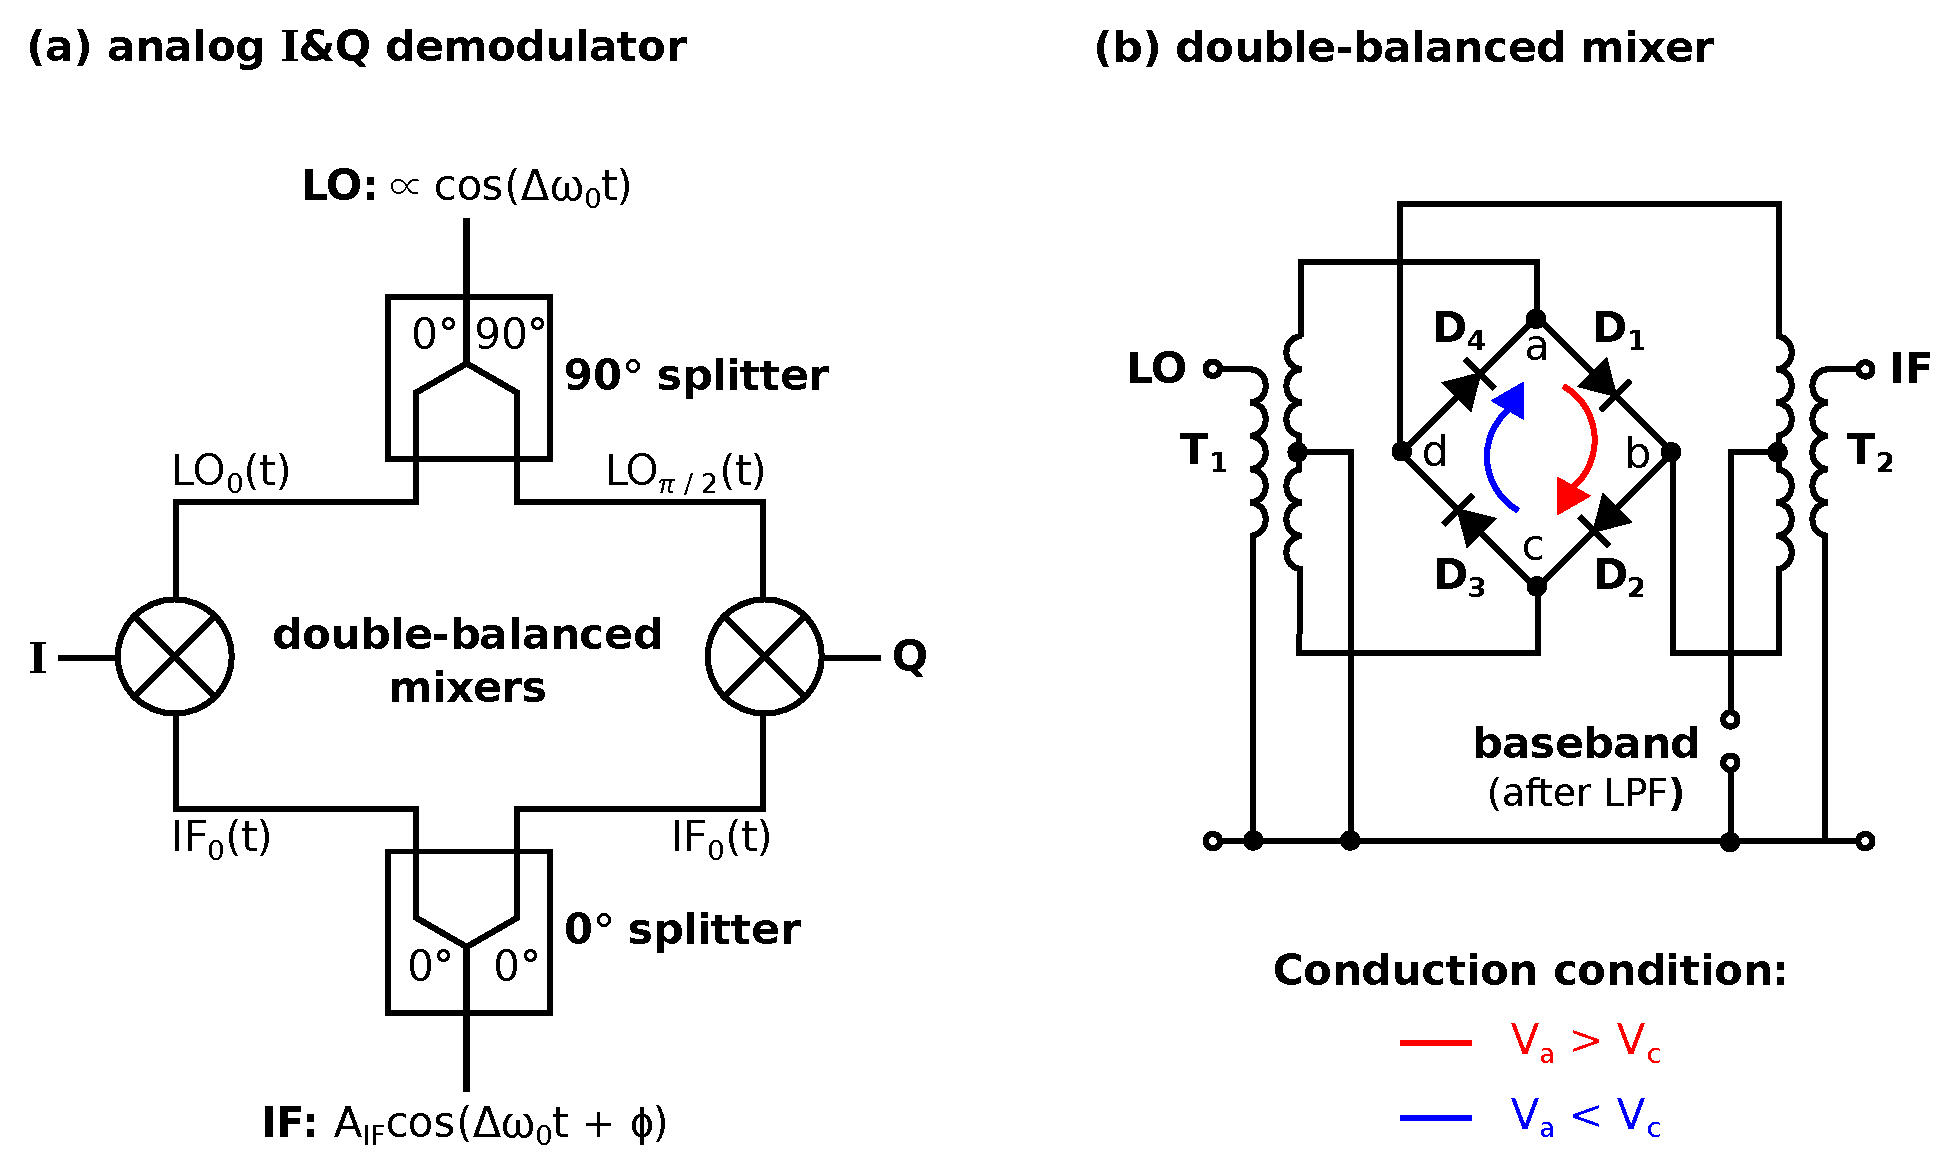
\includegraphics[width = \textwidth]{%
    Chapters/DesignConsiderations/figs/analog_IQ_demodulator.pdf}
  \caption[Components of a typical analog $I\&Q$ demodulator]{%
    (a) A typical analog $I\&Q$ demodulator and
    (b) a typical diode-ring double-balanced mixer.}
  \label{fig:DesignConsiderations:analog_IQ_demodulator}
\end{figure}


\subsection{Nonideal mixing}
\label{sec:DesignConsiderations:demodulation:nonideal_mixing}
In Section~\ref{sec:DesignConsiderations:demodulation:ideal},
mixing was idealized as the multiplication of the IF signal
by a sinusoidal LO signal.
However, in practice, more complex processes are used
to maximize the mixer's linear dynamic range and minimize its noise figure
\cite{analog_devices_mix_and_mod,bryant_mult_vs_mod}.

For example, a typical ring-diode double-balanced mixer
\cite{analog_devices_mix_and_mod}
is shown in Figure~\ref{fig:DesignConsiderations:analog_IQ_demodulator}(b).
The balun transformers $T_1$ and $T_2$
isolate the baseband port from the LO and IF ports.
Typically, the LO power is $\sim \SI{20}{\deci\bel}$ larger than the IF power.
As a result, the LO alone is responsible
for biasing the mixer's diodes into conduction.
Note that the diodes are not all simultaneously biased into conduction.
Instead, when $V_a > V_c$ (neglecting the diode drops),
diodes $D_1$ and $D_2$ are forced into conduction such that
$V_b$ acts as a virtual ground for the IF signal
coupled through transformer $T_2$.
Then, when the LO changes sign such that $V_a < V_c$,
diodes $D_1$ and $D_2$ stop conducting, and
diodes $D_3$ and $D_4$ begin to conduct,
forcing the virtual ground to jump from $V_b$ to $V_d$.
Thus, the ring diode acts as a switch
for the polarization of the coupled IF signal,
with the switching governed by the sign and frequency of the LO.
Low-pass filtering the polarization-modulated IF, of course,
yields the desired baseband signal.
Note that the diode switching time should be minimized
for optimal modulation,
explaining why some manufacturers
advocate the use of a square, rather than a sinusoidal, LO
\cite{minicircuits_mixer_faqs}.

\begin{figure}
  \centering
  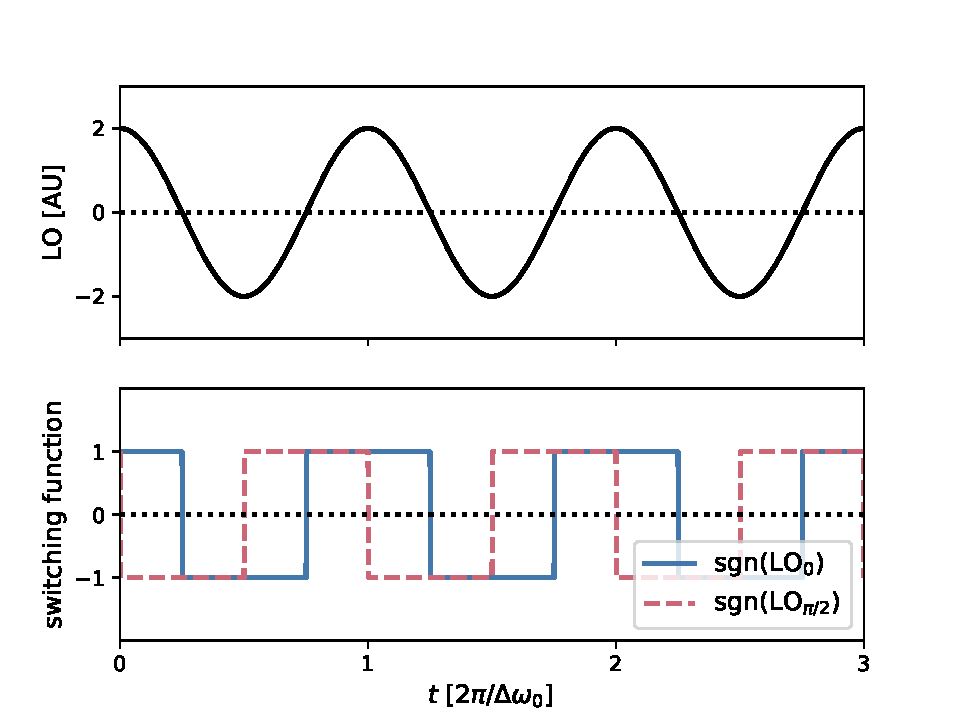
\includegraphics[width = \textwidth]{%
    Chapters/DesignConsiderations/figs/LO_switching_function.pdf}
  \caption[LO switching functions]{%
    The LO switching functions.
    The top panel displays the incident sinusoidal LO signal, while
    the bottom panel shows the \emph{sign} of
    the in-phase ($\text{LO}_0$) and
    the $\pi / 2$ phase-advanced ($\text{LO}_{\pi / 2}$)
    copies of the LO signals.}
  \label{fig:DesignConsiderations:LO_switching_function}
\end{figure}

This polarization modulation can alter the baseband spectrum.
To see this, note that the sign of the in-phase LO signal
is simply a zero-mean square wave with even symmetry about the origin,
as shown in the lower pane of
Figure~\ref{fig:DesignConsiderations:LO_switching_function}.
The Fourier series of such a square wave
consists of a sum over all of the LO's \emph{odd} harmonics:
\begin{align}
  \text{sgn}\left( \text{LO}_0(t) \right)
  &=
  \frac{4}{\pi}
  \sum_{n = 1}^{\infty}
  \frac{(-1)^{n - 1}}{2n - 1} \cos[(2n - 1) \Delta\omega_0 t]
  \\
  &\begin{aligned}
    =
    \frac{4}{\pi}
    \biggl[%
      \cos(\Delta\omega_0 t)
      &-
      \frac{1}{3} \cos(3 \Delta\omega_0 t)
      +
      \cdots
    \biggr].
  \end{aligned}
  \notag
\end{align}
Now, if the IF signal is a perfect sinusoid
as in (\ref{eq:DesignConsiderations:IF_perfect_sinusoid}),
following Section~\ref{sec:DesignConsiderations:demodulation:ideal}'s program
of mixing the LO with the IF and low-pass filtering yields
the desired in-phase baseband signal, e.g.\
\begin{align}
  I
  &=
  \bigl[%
    \text{sgn}\left( \text{LO}_0(t) \right)
    \cdot
    \text{IF}_0(t)
  \bigr]
  \biggr|_{|\omega| \ll \Delta\omega_0}
  \notag \\
  &=
  \frac{\sqrt{2} A_{\text{IF}}}{\pi} \cos\phi
\end{align}
However, if the path from the mixer's IF port to its baseband port
is not wholly linear
(and every real-world device exhibits \emph{some} degree of nonlinearity),
the IF signal will contain contributions from its higher-order harmonics.
If this nonlinearity depends only on the magnitude of the IF
(e.g.\, double-sided saturation/clipping of the signal),
only the odd harmonics of the fundamental will contribute, i.e.\
\begin{equation}
  \text{IF}_0(t)
  =
  \frac{1}{\sqrt{2}}
  \sum_{n = 1}^{\infty}
  A_{2n - 1} \cos\left[ (2n - 1) (\Delta\omega_0 t + \phi) \right],
\end{equation}
where $A_n / \sqrt{2}$ is the Fourier coefficient of the $n\ts{th}$ harmonic
(note that this unconventional normalization facilitates comparison with
the previous, ideal definition of $IF_0(t)$
(\ref{eq:DesignConsiderations:split_IF})).
Typically, $A_n$ decreases as $n$ increases, but
raising the IF amplitude drives more nonlinear interactions and
increases the power in the higher order harmonics relative to the fundamental.
Then,
following Section~\ref{sec:DesignConsiderations:demodulation:ideal}'s program
of mixing the LO with the IF and low-pass filtering yields
\begin{align}
  I
  &=
  \bigl[%
    \text{sgn}\left( \text{LO}_0(t) \right)
    \cdot
    \text{IF}_0(t)
  \bigr]
  \biggr|_{|\omega| \ll \Delta\omega_0}
  \notag \\
  &=
  \frac{\sqrt{2} A_1}{\pi}
  \left[%
    \cos\phi
    -
    \frac{1}{3}\left( \frac{A_3}{A_1} \right) \cos 3 \phi
    +
    \cdots
  \right].
\end{align}
That is, the higher order harmonics of the IF signal
interact with the corresponding higher order harmonics
of the LO switching function
to produce harmonics in the baseband signal.
The coefficient $A_n / (n \cdot A_1)$ gives
the \emph{suppression} of the $n\ts{th}$ harmonic, and
it is typically expressed in decibels
referenced to the power of the carrier, or dBc, as
\begin{equation}
  \text{suppression of $n\ts{th}$ harmonic [dBc]}
  =
  20 \log_{10} \left( \frac{A_n}{n \cdot A_1} \right).
\end{equation}
Noting that $\text{sgn}(\text{LO}_{\pi / 2}(t))$
is an inverted, zero-mean square wave
with \emph{odd} symmetry about the origin,
as shown in the lower pane of
Figure~\ref{fig:DesignConsiderations:LO_switching_function},
a similar path of reasoning to that used above
shows that the quadrature baseband signal is
\begin{align}
  Q
  &=
  \bigl[%
    \text{sgn}\left( \text{LO}_{\pi / 2}(t) \right)
    \cdot
    \text{IF}_0(t)
  \bigr]
  \biggr|_{\omega \ll \Delta\omega_0}
  \notag \\
  &=
  \frac{\sqrt{2} A_1}{\pi}
  \left[%
    \sin\phi
    +
    \frac{1}{3}\left( \frac{A_3}{A_1} \right) \sin 3 \phi
    +
    \cdots
  \right].
\end{align}
Additional distortion of the baseband signal results
if the IF power becomes comparable the LO power,
say within $\SI{10}{\deci\bel}$,
as the IF signal begins to contribute
to the modulation of the diode conduction.

Finally, the diodes of the mixers should be matched as closely as possible.
If, for example, diodes $D_1$ and $D_2$
have slightly different voltage drops than diodes $D_3$ and $D_4$,
the virtual grounds at $V_b$ and $V_d$ are not equivalent
when referenced to ground, and
the resulting baseband signal will have a DC offset.
With precision fabrication, however,
it is not uncommon for the DC offset to be smaller than $1\%$
of the amplitude of the baseband fundamental harmonic.


\subsection{Demodulator imbalances}
\label{sec:DesignConsiderations:demodulation:demodulator_imbalances}
In addition to two double-balanced mixers,
an analog $I\&Q$ demodulator also relies on
a $90^{\circ}$ splitter and a $0^{\circ}$ splitter.
Imbalances between any of these components
can result in imbalances in the baseband $I\&Q$ signals.
For example, unequal power division in the splitters
produces amplitude imbalances in the baseband $I\&Q$ signals, while
deviations from the nominal splitter phasings
produces phase imbalances in the baseband $I\&Q$ signals.
As discussed in
Section~\ref{sec:DesignConsiderations:demodulation:nonideal_mixing},
each double-balanced mixer can produce
spectral distortion and DC offsets in the baseband signal;
in addition, differences between the two mixers
can exacerbate amplitude and phase imbalances
in the baseband $I\&Q$ signals.
Taken all together, then,
the most general form for the baseband $I\&Q$ signals is
\begin{align}
  I
  &=
  I_1 \left\{%
    \cos\phi
    -
    \frac{I_3}{3 I_1}
    \cos \left( 3 \phi \right)
    +
    \cdots
  \right\}
  +
  \delta I,
  \label{eq:DesignConsiderations:I_general}
  \\
  Q
  &=
  Q_1 \left\{%
    \sin \left( \phi + \delta \right)
    +
    \frac{Q_3}{3 Q_1}
    \sin \left[ 3 \left( \phi + \delta \right) \right]
    +
    \cdots
  \right\}
  +
  \delta Q,
  \label{eq:DesignConsiderations:Q_general}
\end{align}
where
$I_1$ is the amplitude of the in-phase signal's fundamental harmonic,
$I_3$ is the amplitude of the in-phase signal's third harmonic, and
$\delta I$ is the in-phase signal's DC offset.
Similar nomenclature applies to the quadrature signal.
The phase imbalance of the demodulator is $\delta$.
Amplitude imbalances occur when $I_1 \neq Q_1$.
The harmonic suppressions are typically comparable,
e.g.\ $|I_3 / I_1| \approx |Q_3 / Q_1|$.
Note that (\ref{eq:DesignConsiderations:I_general}) and
(\ref{eq:DesignConsiderations:Q_general})
generalize previous forms for the $I\&Q$ signals
\cite{vanzeeland_rsi04}.


\subsection{Effects of demodulator imperfections}
\label{sec:DesignConsiderations:demodulation:imperfection_implications}
Demodulator imperfections produce systematic errors
in the measured phase~\cite{vanzeeland_rsi04,kasten_masters}.
Specifically, if the $I\&Q$ signals suffer from imbalances and nonlinearities,
as shown in (\ref{eq:DesignConsiderations:I_general}) and
(\ref{eq:DesignConsiderations:Q_general}),
then the measured phase $\phi_m$ computed via the inverse tangent formula
(\ref{eq:DesignConsiderations:phase_from_arctangent})
will \emph{not} correspond to the true phase $\phi$, i.e.\
\begin{equation}
  \phi_m = \phi + \delta \phi,
\end{equation}
where $\delta\phi$ is the error in the measured phase.
The phase error is a complicated, periodic function of the true phase,
i.e.\ $\delta\phi = \delta\phi(\phi)$~\cite{vanzeeland_rsi04}.
For small phase fluctuations $|\tilde{\phi}| \ll 1$
about an equilibrium phase $\bar{\phi}$,
the error $\delta\tilde{\phi}$ in the measured fluctuating phase
is simply the \emph{change} in the total phase error
between $\bar{\phi}$ and $\bar{\phi} + \tilde{\phi}$
\cite{kasten_masters}:
\begin{equation}
  \delta\tilde{\phi}
  =
  \delta\phi(\bar{\phi} + \tilde{\phi}) - \delta\phi(\bar{\phi})
  \approx
  \left[%
    \left. \frac{d(\delta\phi)}{d\phi} \right|_{\bar{\phi}}
  \right] \tilde{\phi}.
\end{equation}
Thus, the \emph{relative} error in the measured fluctuating phase is
\begin{equation}
  \frac{\delta\tilde{\phi}}{\tilde{\phi}}
  =
  \left. \frac{d(\delta\phi)}{d\phi} \right|_{\bar{\phi}}.
  \label{eq:DesignConsiderations:relative_fluctuation_error}
\end{equation}
Synthetic $I\&Q$ Lissajous curves and
the relative errors in the measured fluctuating phase
that result from various demodulator imperfections
are displayed in
Figure~\ref{fig:DesignConsiderations:effects_of_demodulator_imperfections}.
Obviously, each demodulator imperfection should be minimized
in order to minimize the relative error
in the measured fluctuating phase.

\begin{figure}
  \centering
  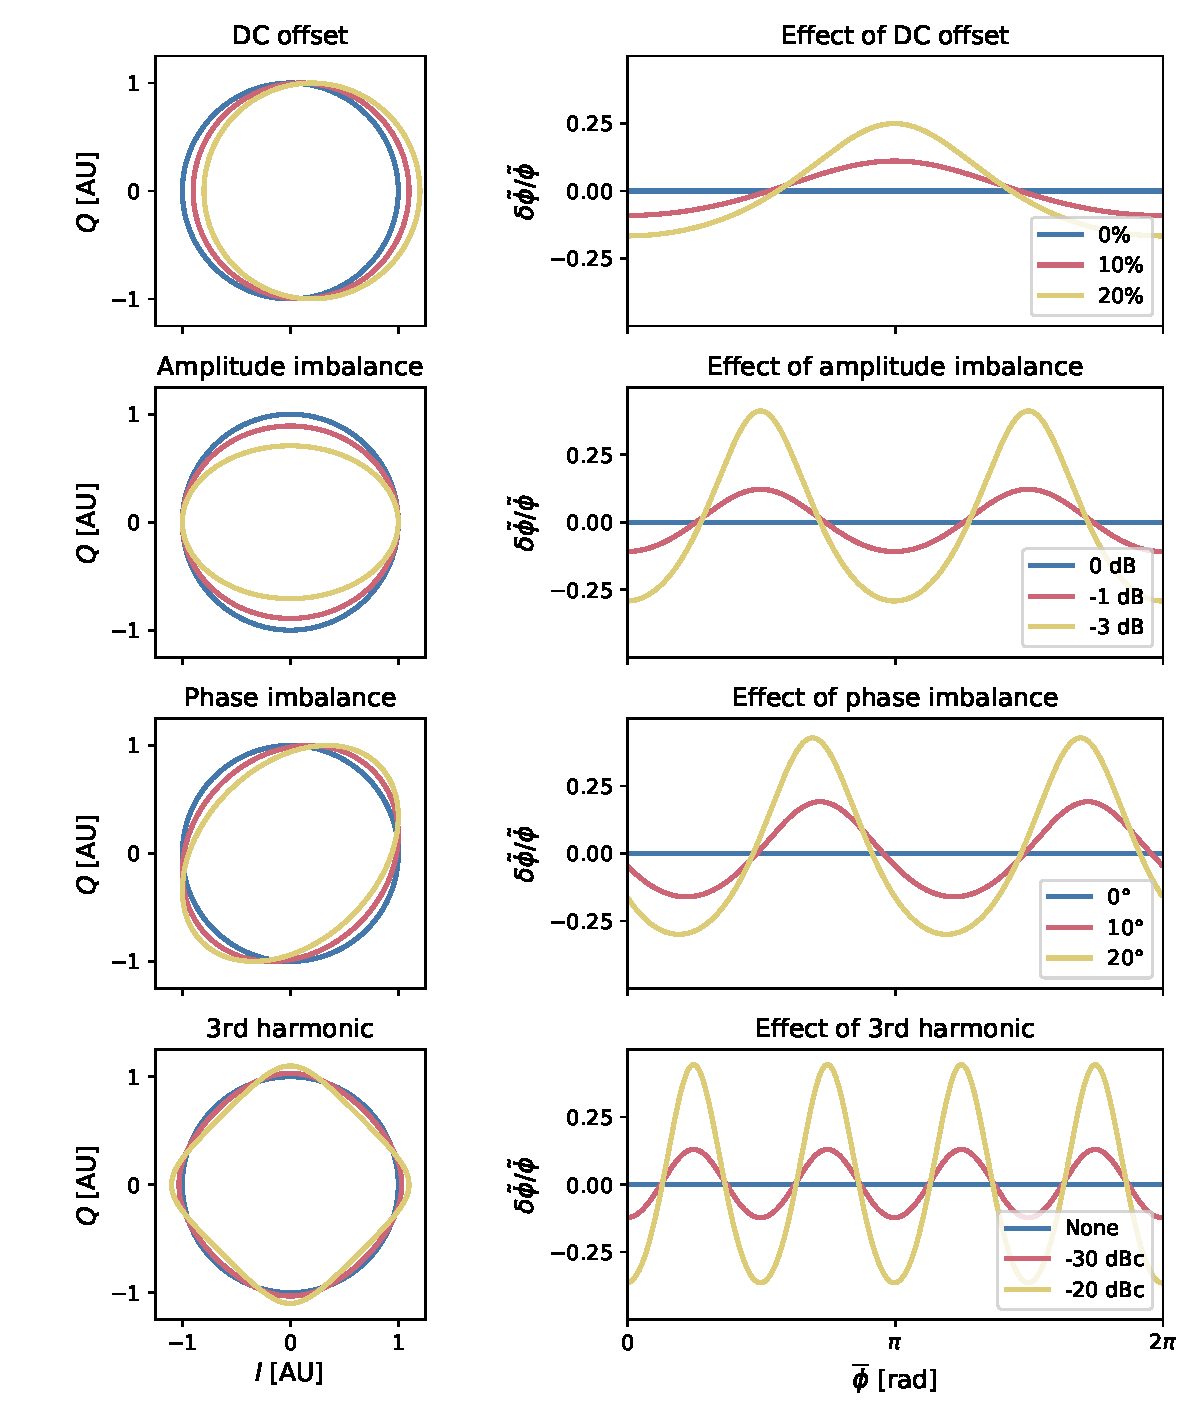
\includegraphics[width = \textwidth]{%
    Chapters/DesignConsiderations/figs/demodulator_imperfections.pdf}
  \caption[Effects of demodulator imperfections]{%
    Demodulator imperfections produce errors in the measured phase.
    The left column displays the Lissajous curves
    that result from plotting
    synthetic quadrature $Q$ vs.\ in-phase $I$ signals, while
    the right column plots the relative error
    $\delta\tilde{\phi} / \tilde{\phi}$
    in the measured fluctuating phase
    as a function of the equilibrium phase $\bar{\phi}$.
    Each row examines a different demodulator imperfection.
  }
  \label{fig:DesignConsiderations:effects_of_demodulator_imperfections}
\end{figure}


\section{Quantization noise}
\label{sec:DesignConsiderations:quantization}
Efficient conversion of an analog signal to a digital record requires
quantization of the signal magnitude and
temporal sampling of these quantized magnitudes~\cite{bennett_bstj48}.
This analog-to-digital conversion
is performed by an instrument known as a digitizer.
If a digitizer has bit depth $N_b$ and
an input-voltage dynamic range $V_{\text{dyn}}$,
then its quantum of voltage $\Delta V$ is
\begin{equation}
  \Delta V
  =
  \frac{V_{\text{dyn}}}{2^{N_b} - 1}
  \approx
  \frac{V_{\text{dyn}}}{2^{N_b}},
  \label{eq:DesignConsiderations:digitizer_voltage_quantum}
\end{equation}
where the approximation is well-satisfied
for typical digitizer bit depths.
At each sampling time,
the analog signal's magnitude is approximated
by the closest quantized value, whose
separation from the true, analog value
will be less than or equal to $\Delta V / 2$.

In general, then, the quantized signal
will differ from the analog signal.
This error $\epsilon$ is known as quantization noise.
The mean square error (i.e.\ variance) attributable to quantization is simply
\begin{equation}
  \overline{\epsilon^2} = \frac{(\Delta V)^2}{12},
  \label{eq:DesignConsiderations:quantization_noise_variance}
\end{equation}
where $\Delta V$ is the digitizer's quantum of voltage,
as given by (\ref{eq:DesignConsiderations:digitizer_voltage_quantum})
\cite{bennett_bstj48}
\cite[Sec.~10.2.4]{bendat_and_piersol}.
For a uniformly sampled record with sampling rate $f_s$,
sufficiently fine quantization $\Delta V$
ensures that the quantization noise is \emph{white}
\cite[Th.~1]{bennett_bstj48}
\cite[Ch.~20]{widrow_and_kollar};
that is, the one-sided autospectral density of the quantization noise is
\begin{align}
  G_{\epsilon,\epsilon}(f)
  =
  \frac{\overline{\epsilon^2}}{f_s / 2}
  =
  \frac{(\Delta V)^2}{6 f_s},
  \qquad
  0 \leq f \leq \frac{f_s}{2}.
  \label{eq:DesignConsiderations:quantization_noise_autospectral_density}
\end{align}
In practice, however, aperture error, jitter, and nonlinearities
may reduce the effective bit depth by one or two bits
\cite[Sec.~10.2.4]{bendat_and_piersol},
increasing the realized quantization noise
relative to that expected from
(\ref{eq:DesignConsiderations:quantization_noise_variance}) and
(\ref{eq:DesignConsiderations:quantization_noise_autospectral_density}).

Quantization noise can be significant
when attempting to measure absolute phase fluctuations
with a heterodyne interferometer.
Recall from the discussion of heterodyne interferometric detection in
Section~\ref{sec:InterferometricMethods:interferometry:heterodyne}
that measurement of the \emph{absolute} phase
requires capturing the full dynamics
of the large, slowly varying equilibrium phase $\bar{\phi}$
in addition to measuring the fluctuating phase $\tilde{\phi}$.
Because $\tilde{\phi} \ll \bar{\phi}$ in typical situations,
the fluctuations only occupy a small portion
of the digitizer's dynamic range; that is,
fluctuations effectively see a bit depth that
is substantially smaller than the digitizer's nominal bit depth.
Thus, to minimize the effect of quantization noise,
it is absolutely imperative
to utilize the full dynamic range of the digitizer.

The measured phase $\phi_m$ is computed from
the in-phase ($I$) and quadrature ($Q$) signals via
(\ref{eq:DesignConsiderations:phase_from_arctangent}).
If needed for feedback control,
the phase can be calculated in real time
with analog or digital electronics.
If the real-time phase is not needed,
it is sufficient to digitize the $I$ and $Q$ signals individually;
later, offline, the phase can be computed in software.
In the offline approach,
software may additionally compensate demodulator imperfections
(discussed in Section~\ref{sec:DesignConsiderations:demodulation})
prior to computing the phase.
Of course, the offline approach
subjects both the $I$ and the $Q$ signal to quantization noise.
The quantization error $\varepsilon_I$ of $I$ and
the quantization error $\varepsilon_Q$ of $Q$
are uncorrelated, so
the total one-sided autospectral density of the quantization noise is simply
the sum of the individual one-sided autospectral densities, i.e.\
\begin{equation}
  G_{\epsilon_I,\epsilon_I}(f)
  +
  G_{\epsilon_Q,\epsilon_Q}(f)
  =
  \frac{(\Delta V)^2}{3 f_s},
  \qquad
  0 \leq f \leq \frac{f_s}{2}.
  \label{eq:DesignConsiderations:total_quantization_noise_autospectral_density}
\end{equation}
Note that comparing the spectral density of the quantization noise
to the spectral density of the measured phase
(with the phase having units of radians)
requires converting
(\ref{eq:DesignConsiderations:total_quantization_noise_autospectral_density})
from units of $\SI{}{\volt\squared\per\Hz}$
to the corresponding angular equivalent.
This unit conversion is accomplished by dividing
(\ref{eq:DesignConsiderations:total_quantization_noise_autospectral_density})
by the \emph{squared} radius of the $I\&Q$ Lissajous curve.
Let the $I$ and $Q$ signals occupy
a fraction $\eta_{\text{dyn}} \leq 1$ of
the digitizer's full dynamic range $V_{\text{dyn}}$ such that
the squared radius of the Lissajous curve is
$I^2 + Q^2 = (\eta_{\text{dyn}} V_{\text{dyn}} / 2)^2$, and
the total quantization noise
(in angular units of $\SI{}{\radian\squared\per\Hz}$) is
\begin{equation}
  G_{\epsilon_I,\epsilon_I}(f)
  +
  G_{\epsilon_Q,\epsilon_Q}(f)
  \approx
  \frac{1}{3 \left[ 2^{2 (N_b - 1)} \right] \eta_{\text{dyn}}^2 f_s},
  \quad
  0 \leq f \leq \frac{f_s}{2},
  \label{eq:DesignConsiderations:total_quantization_noise_autospectral_density_angular_units}
\end{equation}
where the definition of the voltage quantum
(\ref{eq:DesignConsiderations:digitizer_voltage_quantum})
has been utilized.


\section{Summary}
\label{sec:DesignConsiderations:summary}
For ease of reference, this section provides a concise summary
of the design considerations discussed in this chapter.
If more details are desired regarding any given design consideration,
the summary also points to the appropriate section in the text.


\subsection{Geometric considerations}
The measurements of a heterodyne interferometer
are influenced by several geometric effects,
which are summarized below:
\begin{itemize}
  \item \emph{Aperture diffraction} can alter the propagation
    of the unscattered and scattered Gaussian beams
    that formed the basis of the analysis in
    Chapter~\ref{ch:InterferometricMethods}.
    Aperture diffraction of a Gaussian beam is minimal if
    \begin{equation}
      a_{\text{eff}} \geq \frac{3}{2} w(z),
      \label{eq:DesignConsiderations:summary:aperture_radius_for_minimal_diffraction}
    \end{equation}
    for each aperture, where
    $a_{\text{eff}}$ is the effective aperture radius and
    $w(z)$ is the beam's 1/e $E$ radius at the aperture location.
    For a beam located transverse distance
    $\rho(z)$ away from the optical axis,
    a circular aperture of radius $a$ has
    an effective aperture radius $a_{\text{eff}} = a - |\rho(z)|$.
    See Section~\ref{sec:DesignConsiderations:geometric:aperture_diffraction}
    for more details.
  \item \emph{Beam coalignment} affects
    the size of the interference signal.
    If the reference beam and the unscattered probe beam
    are misaligned by angle $\theta$,
    then obtaining a finite interference signal
    from a detector element of length $s_x$
    requires that
    \begin{equation}
      |\theta|
      \ll
      \frac{\lambda_0}{s_x}
      \approx
      0.6^{\circ},
      \label{eq:DesignConsiderations:summary:coalignment_constraint}
    \end{equation}
    where $\lambda_0 = 2 \pi / k_0$ is the beam wavelength,
    and the typical values
    $\lambda_0 = \SI{10.6}{\micro\meter}$ and
    $s_x = \SI{1}{\milli\meter}$
    have been used for the evaluation.
    See Section~\ref{sec:DesignConsiderations:geometric:beam_coalignment}
    for more details.
  \item \emph{Differences in the radii of curvature}
    between the reference beam and the probe beam
    can alter the interference pattern at the detector,
    potentially decreasing the size of the interference signal and
    distorting the imaged wavenumbers.
    These detrimental curvature effects are negligible if
    \begin{equation}
      \text{max}(\delta\phi_{\kappa})
      =
      \frac{k_0}{8}
      \left[ (N_{\text{el}} s_x)^2 + s_y^2 \right]
      \left| \frac{1}{R_P(z_{\image})} - \frac{1}{R_R(z_R)}\right|
      \ll
      \pi.
      \label{eq:DesignConsiderations:summary:radii_of_curvature_matching}
    \end{equation}
    where
    $R_P(z_{\image})$ is the radius of curvature
    of the probe beam at the detector location,
    $R_R(z_R)$ is the radius of curvature
    of the reference beam at the detector location,
    $k_0$ is the wavenumber of the probe radiation,
    $s_x$ and $s_y$ are the linear dimensions
    of a single detector element in the $x$- and $y$-dimensions, respectively,
    and $N_{\text{el}}$ is the number of such detector elements
    (arranged in the $x$-direction with negligible inter-element spacing).
    See Section~\ref{sec:DesignConsiderations:geometric:beam_mismatch}
    for more details.
  \item The \emph{finite sampling-volume effect} introduces
    a wavenumber dependence into the transfer function
    of a heterodyne interferometer.
    See Section~\ref{sec:DesignConsiderations:summary:wavenumber_transfer_function}
    for a summary of this effect;
    see Section~\ref{sec:DesignConsiderations:geometric:finite_sampling_volume}
    for additional details.
  \item The \emph{depth of focus} is the axial distance by which
    the detector location may deviate from the image plane.
    If $\delta z_{\image}$ is the axial displacement
    of the detector from the image plane
    (i.e. $z_{\text{det}} = z_{\image} + \delta z_{\image}$),
    a heterodyne interferometer will measure wavenumbers $k_{\text{meas}}$
    that are biased away from their true values $k$ by
    \begin{equation}
      k_{\text{meas}}
      =
      \left[
        1
        -
        \frac{\delta z_{\image}}{R(z_{\text{det}})}
      \right]
      k,
      \label{eq:DesignConsiderations:summary:depth_of_focus_wavenumber_distortion}
    \end{equation}
    where $R(z_{\text{det}})$ is the radius of curvature of the probe beam
    at the detector.
    Additionally, the ``out-of-focus'' interference
    of the upscattered and downscattered beams
    produces a wavenumber-dependent phase shift
    \begin{equation}
      \mu
      =
      \left( \frac{k^2}{2 M^2 k_0} \right) \delta z_{\image},
      \label{eq:DesignConsiderations:summary:depth_of_focus_wavenumber_dependent_phase_shift}
    \end{equation}
    where $M$ is the magnification of the imaging system and
    $k_0$ is the wavenumber of the probe radiation.
    Autospectral densities of the phase fluctuations
    can be computed independent of $\mu$, but
    it is less clear how to compute e.g.\
    cross-spectral densities or bispectral densities
    in a $\mu$-independent manner.
    An imaging system should be designed
    such that reasonable uncertainties in $\delta z_{\image}$
    produce negligible wavenumber distortion
    (i.e.\ $|\delta z_{\image} / R(z_{\text{det}})| \ll 1$) and
    negligible wavenumber-dependent phase shifts (i.e. $|\mu| \ll 1$).
    See Section~\ref{sec:DesignConsiderations:geometric:depth_of_focus}
    for more details.
\end{itemize}


\subsection{Wavenumber transfer function}
\label{sec:DesignConsiderations:summary:wavenumber_transfer_function}
The heterodyne interferometer's basic wavenumber transfer function
(derived in Chapter~\ref{ch:InterferometricMethods})
is modified by several design decisions, becoming
\begin{equation}
  T_{\text{het}}(k)
  =
  \frac{1}{\sqrt{2} \pi}
  \cdot
  \frac{2 I_{\text{AC}}}{I_{\text{DC}} + I_{\text{AC}}}
  \cdot
  \frac{V_1}{V_1(I_{\text{max}} = I_{\text{sat}})}
  \cdot
  T_{\text{fsv}}(k),
  \label{eq:DesignConsiderations:summary:heterodyne_interferometer_wavenumber_transfer_function}
\end{equation}
where
\begin{itemize}
  \item The first term $1 / (\sqrt{2} \cdot \pi)$
    corresponds to the heterodyne interferometer's
    basic wavenumber transfer function
    (\ref{eq:InterferometricMethods:heterodyne_interferometer_wavenumber_transfer_function}).
    See Section~\ref{sec:InterferometricMethods:interferometry:heterodyne}
    for more details.
  \item The second term $2 I_{\text{AC}} / (I_{\text{DC}} + I_{\text{AC}})$
    specifies the ratio of peak-to-peak AC intensity to the maximum intensity
    in the heterodyne interference signal, where
    the DC intensity $I_{\text{DC}}$ is defined by
    (\ref{eq:DesignConsiderations:I_DC}) and
    the AC intensity $I_{\text{AC}}$ is defined by
    (\ref{eq:DesignConsiderations:I_AC}).
    This modification to the transfer function
    is maximized when $I_{\text{DC}} = I_{\text{AC}}$, i.e.\
    when there is full-depth modulation of the heterodyne intensity, which
    occurs when the probe beam and reference beam
    have identical spatial structures and powers.
    See Section~\ref{sec:DesignConsiderations:geometric:beam_mismatch}
    for more details.
  \item The third term $V_1 / V_1(I_{\text{max}} = I_{\text{sat}})$
    specifies the ratio of the realized amplitude (in volts) $V_1$
    of the IF signal's fundamental harmonic
    relative to the corresponding amplitude
    $V_1(I_{\text{max}} = I_{\text{sat}})$
    when the maximum incident intensity $I_{\text{max}}$
    is scaled to the detector's saturation intensity $I_{\text{sat}}$
    (the AC and DC fractions of the incident intensity
    are \emph{not} altered during this scaling;
    to account for changing the AC and DC fractions,
    see the transfer function's second term,
    $2 I_{\text{AC}} / (I_{\text{DC}} + I_{\text{AC}})$).
    Thus, operation above the saturation intensity \emph{may} increase
    the heterodyne interferometer's wavenumber transfer function
    (i.e.\ if $V_1 > V_1(I_{\text{max}} = I_{\text{sat}})$, where
    $V_1$ depends sensitively on the detector's saturation physics).
    Similarly, operating below the saturation intensity will decrease
    the heterodyne interferometer's wavenumber transfer function.
    (i.e.\ $V_1 < V_1(I_{\text{max}} = I_{\text{sat}})$).
    See Section~\ref{sec:DesignConsiderations:intensity}
    for more details.
  \item The fourth and final term $T_{\text{fsv}}(k)$
    quantifies the effect of sampling the interfering radiation field
    with detector elements of \emph{finite} size.
    The output of each detector element
    corresponds to the incident intensity
    \emph{averaged} over the element's active area, and
    this averaging acts as a low-pass filter in the spatial domain.
    This is referred to as the \emph{finite sampling-volume effect}, and
    a square detector of linear dimension $s_x$
    placed in the image plane of a magnification $M$ imaging system
    has the corresponding transfer function
    \begin{equation}
      T_{\text{fsv}}(k)
      =
      \sinc\left( \frac{k}{k_{\text{fsv}}} \right),
      \label{eq:DesignConsiderations:summary:finite_sampling_volume_transfer_function}
    \end{equation}
    where
    \begin{equation}
      \sinc(x) = \frac{\sin(\pi x)}{\pi x}
      \label{eq:DesignConsiderations:summary:normalized_sinc}
    \end{equation}
    is the normalized sinc function, and
    \begin{equation}
      k_{\text{fsv}} = \frac{2 \pi |M|}{s_x}
      \label{eq:DesignConsiderations:summary:finite_sampling_volume_cutoff}
    \end{equation}
    is the first zero of $T_{\text{fsv}}(k)$.
    Wavenumbers $|k| \lesssim k_{\text{fsv}}$ are measurable, while
    wavenumbers $|k| \gtrsim k_{\text{fsv}}$ are not measurable.
    See Section~\ref{sec:DesignConsiderations:geometric:finite_sampling_volume}
    for more details.
    The finite sampling-volume effect is exploited
    in Chapter~\ref{ch:Implementation}
    to provide an overlap in the wavenumber sensitivities
    of \diiid's pre-existing phase contrast imaging (PCI) system and
    its newly installed heterodyne interferometer.
\end{itemize}


\subsection{The measured phase}
An absolute phase measurement $\phi_m$ is
computed from a heterodyne interferometer's
demodulated in-phase ($I$) and quadrature ($Q$) signals via
\begin{equation}
  \phi_m = \atantwo\left(Q, I\right),
  \label{eq:DesignConsiderations:summary:phase_from_arctangent}
\end{equation}
where $\atantwo\left(Q, I\right)$
is the arctangent function of two arguments, which
uses the signs of $Q$ and $I$ to correctly determine
the quadrant corresponding to the tangent of $Q / I$.
Demodulator imperfections
produce a systematic error $\delta \phi$ in the measured phase, i.e.\
\begin{equation}
  \phi_m = \phi + \delta \phi,
  \label{eq:DesignConsiderations:summary:phase_error}
\end{equation}
where $\phi$ is the true phase.
This systematic error is a complicated,
periodic function of the true phase, i.e.\
$\delta \phi = \delta \phi(\phi)$.
For small phase fluctuations $|\tilde{\phi}| \ll 1$
about an equilibrium phase $\bar{\phi}$,
the \emph{relative} error in the measured fluctuating phase is
\begin{equation}
  \frac{\delta\tilde{\phi}}{\tilde{\phi}}
  =
  \left. \frac{d(\delta\phi)}{d\phi} \right|_{\bar{\phi}}.
  \label{eq:DesignConsiderations:summary:relative_fluctuation_error}
\end{equation}
See Section~\ref{sec:DesignConsiderations:demodulation}
for more details.


\subsection{Noise sources \& their spectral densities}
\label{sec:DesignConsiderations:summary:noise}
The phase measurements of a heterodyne interferometer can be corrupted by
oscillator phase noise, optical shot noise, electrical noise, and
quantization noise.
The origins and the spectral densities of these noise sources
are summarized below:
\begin{itemize}
  \item \emph{Laser phase noise}
    $\mathcal{L}_{\omega_0}(f)$
    injects noise into a heterodyne interferometer's measurements.
    The one-sided autospectral density of this noise is
    \begin{equation}
      G(f)
      =
      8 \sin^2(\pi f \tau) \mathcal{L}_{\omega_0}(f),
      \qquad
      f \geq 0,
      \label{eq:DesignConsiderations:summary:laser_phase_noise_autospectral_density}
    \end{equation}
    where $\tau = L / c$ is the time delay
    associated with the optical path-length difference $L$
    between the interferometer's probe arm and reference arm.
    See Section~\ref{sec:DesignConsiderations:phase_noise:laser}
    for more details.
  \item \emph{Local oscillator (LO) phase noise}
    $\mathcal{L}_{\Delta \omega_0}(f)$
    injects noise into a heterodyne interferometer's measurements.
    The one-sided autospectral density of this noise is
    \begin{equation}
      G(f)
      =
      8 \sin^2(\pi f \tau) \mathcal{L}_{\Delta \omega_0}(f),
      \qquad
      f \geq 0,
      \label{eq:DesignConsiderations:summary:LO_phase_noise_autospectral_density}
    \end{equation}
    where $\tau$ is the time required to couple the LO signal
    to the interferometer's Doppler-shifted beam.
    See Section~\ref{sec:DesignConsiderations:phase_noise:LO}
    for more details.
  \item \emph{Detector noise} near the intermediate frequency $\Delta f_0$
    is demodulated and contaminates a heterodyne interferometer's measurements.
    The one-sided autospectral density of the demodulated detector noise
    (in angular units of $\SI{}{\radian\squared\per\Hz}$) is
    \begin{equation}
      G(f)
      =
      \frac{A}{P_P P_R (D^*)^2},
      \qquad
      0 \leq f \ll \Delta f_0,
      \label{eq:DesignConsiderations:summary:detector_noise_autospectral_density}
    \end{equation}
    where $A$ is the area of the detector element,
    $P_P$ is the optical power of the probe beam
    impinging on the detector element,
    $P_R$ is the optical power of the reference beam
    impinging on the detector element,
    and $D^*$ is the specific detectivity of the detector near $\Delta f_0$.
    Here, it is assumed that the probe beam and the reference beam
    vary weakly over the face of the detector element.
    See Section~\ref{sec:DesignConsiderations:amplitude_noise:detector}
    for more details.
  \item \emph{Optical shot noise} is demodulated and
    contaminates a heterodyne interferometer's measurements.
    The one-sided autospectral density
    of the demodulated optical shot noise
    (in angular units of $\SI{}{\radian\squared\per\Hz}$) is
    \begin{equation}
      G(f)
      =
      2 h f_0 \left( \frac{P_P + P_R}{P_P P_R} \right),
      \qquad
      0 \leq f \ll \Delta f_0,
      \label{eq:DesignConsiderations:summary:shot_noise_autospectral_density}
    \end{equation}
    where $h$ is the Planck constant,
    $f_0$ is the frequency of the incident photons,
    $P_P$ is the optical power of the probe beam
    impinging on the detector element,
    $P_R$ is the optical power of the reference beam
    impinging on the detector element, and
    $\Delta f_0$ is the intermediate frequency of the heterodyne signal.
    Here, it is assumed that the probe beam and the reference beam
    vary weakly over the face of the detector element.
    See Section~\ref{sec:DesignConsiderations:amplitude_noise:shot}
    for more details.
  \item \emph{Amplifier noise} is characterized via a noise figure ($NF$),
    which quantifies the degradation in signal-to-noise ratio ($SNR$)
    after passing through the amplifier.
    See Section~\ref{sec:DesignConsiderations:amplitude_noise:amplifier}
    for more details.
  \item \emph{Quantization noise} is produced
    by the creation of a digital record.
    Assuming that the $I$ and $Q$ signals of a heterodyne interferometer
    are individually digitized with bit depth $N_b$ and
    sample rate $f_s$ (in \SI{}{\hertz}),
    the one-sided autospectral density of the total quantization noise
    (in angular units of \SI{}{\radian\squared\per\hertz}) is
    \begin{equation}
      G(f)
      \approx
      \frac{1}{3 \left[ 2^{2 (N_b - 1)} \right] \eta_{\text{dyn}}^2 f_s},
      \qquad
      0 \leq f \leq \frac{f_s}{2},
      \label{eq:DesignConsiderations:summary:quantization_noise_autospectral_density}
    \end{equation}
    where $\eta_{\text{dyn}} \leq 1$ is the fraction
    of the digitizers's dynamic range $V_{\text{dyn}}$
    occupied by the $I$ and $Q$ signals, i.e.\
    \begin{equation}
      \eta_{\text{dyn}}
      =
      \frac{\text{max}(I) - \text{min}(I)}{V_{\text{dyn}}}
      =
      \frac{\text{max}(Q) - \text{min}(Q)}{V_{\text{dyn}}}.
      \label{eq:DesignConsiderations:summary:eta_dynamic}
    \end{equation}
    See Section~\ref{sec:DesignConsiderations:quantization}
    for more details.
\end{itemize}


\bibliographystyle{plainurl}
\bibliography{references}
